%% ============================================================
%% pynasonde — Graduate Student Workshop
%% Beamer presentation (compile with: make tutorials)
%%
%% Manual:
%%   cd tutorials/grad_student
%%   pdflatex pynasonde_workshop.tex
%% ============================================================
\documentclass[aspectratio=169,11pt]{beamer}

% ---------- theme ------------------------------------------------
\usetheme{Madrid}
\usecolortheme{seahorse}
\setbeamertemplate{navigation symbols}{}
\setbeamertemplate{footline}[frame number]
\setbeamerfont{frametitle}{size=\large,series=\bfseries}

% ---------- packages ------------------------------------------------
\usepackage{amsmath,amssymb}
\usepackage{graphicx}
\usepackage{listings}
\usepackage{xcolor}
\usepackage{booktabs}
\usepackage{hyperref}
\usepackage{tikz}
\usetikzlibrary{arrows.meta,positioning,shapes,fit,backgrounds}
\pgfdeclarelayer{background}
\pgfsetlayers{background,main}

% ---------- figure path (relative to this .tex file) ---------------
\graphicspath{{../../docs/examples/figures/}}

% ---------- code style ------------------------------------------------
\definecolor{codebg}{RGB}{245,245,250}
\definecolor{codekw}{RGB}{0,0,180}
\definecolor{codestr}{RGB}{160,32,32}
\definecolor{codecom}{RGB}{0,128,0}

\lstset{
  language=Python,
  backgroundcolor=\color{codebg},
  basicstyle=\ttfamily\footnotesize,
  keywordstyle=\color{codekw}\bfseries,
  stringstyle=\color{codestr},
  commentstyle=\color{codecom}\itshape,
  showstringspaces=false,
  breaklines=true,
  frame=single,
  framerule=0.4pt,
  rulecolor=\color{gray!40},
  xleftmargin=6pt,xrightmargin=6pt,
}

% ---------- title info -----------------------------------------------
\title[pynasonde Workshop]{%
  \textbf{pynasonde} — Ionosonde Data Analysis in Python}
\subtitle{A Hands-On Workshop for Graduate Students}
\author{Ionospheric Remote Sensing Group}
\institute{VIPIR \& DIGISONDE Analysis Toolkit}
\date{\today}

% =================================================================
\begin{document}
% =================================================================

\begin{frame}
  \titlepage
  \vspace{-0.5cm}
  \begin{center}
    \small
    \texttt{pip install pynasonde} \quad|\quad
    \href{https://github.com/shibaji7/pynasonde}{github.com/shibaji7/pynasonde}
  \end{center}
\end{frame}

\begin{frame}{Outline}
  \tableofcontents
\end{frame}

% ----------------------------------------------------------------
\section{Background}
% ----------------------------------------------------------------

\begin{frame}{What is an Ionosonde?}
\begin{columns}
\column{0.6\textwidth}
  \begin{itemize}
    \item A \textbf{pulsed HF radar} ($\sim$1–30~MHz) transmitting vertically
    \item Each frequency reflects at the height where $f_p(h) = f$
    \item Records: virtual height $h'(f)$ vs frequency — the \textbf{ionogram}
    \item \textbf{Two instruments} in this toolkit:
      \begin{itemize}
        \item \textbf{VIPIR} — 8-channel digital receiver, raw IQ storage
        \item \textbf{DIGISONDE DPS4D} — SAO/RSF/DFT/DVL file formats
      \end{itemize}
  \end{itemize}
\column{0.38\textwidth}
  \begin{block}{Key quantities}
    \begin{tabular}{ll}
      $f$     & sounding frequency \\
      $h'(f)$ & virtual height (km)\\
      $f_p$   & plasma frequency \\
      $N(h)$  & electron density \\
    \end{tabular}
  \end{block}
\end{columns}
\end{frame}

\begin{frame}{Two Instrument Families}
  \begin{columns}
  \column{0.48\textwidth}
    \begin{block}{VIPIR}
      \begin{itemize}\small
        \item Grubb et al.\ (2011)
        \item Raw IQ binary (\texttt{.RIQ})
        \item 8 Rx channels, pulse-compressed
        \item Gate spacing: 1.499~km (WI937)
        \item 4 pulses/frequency (typical)
        \item Full analysis: Es imaging, N(h), absorption
      \end{itemize}
    \end{block}
  \column{0.48\textwidth}
    \begin{block}{DIGISONDE DPS4D}
      \begin{itemize}\small
        \item Reinisch et al.\ (1997)
        \item Scaled data: \texttt{.SAO}
        \item Raw soundings: \texttt{.RSF}, \texttt{.SBF}
        \item Doppler spectra: \texttt{.DFT}
        \item Drift velocities: \texttt{.DVL}
        \item Sky maps: \texttt{.SKY}
      \end{itemize}
    \end{block}
  \end{columns}
\end{frame}

%% ---- v1.0 Architecture ----
\begin{frame}{pynasonde v1.0 Architecture (Chakraborty et al., \textit{SoftwareX} 2026)}
\vspace{-0.2cm}
\begin{center}
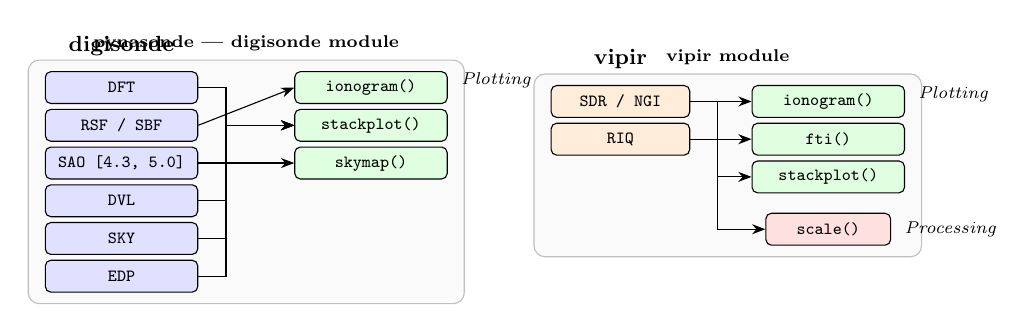
\begin{tikzpicture}[
  >=Stealth,
  every node/.style={font=\scriptsize},
  dnode/.style={draw,fill=blue!12,rounded corners=2pt,
                minimum width=2.2cm,minimum height=0.46cm,align=center},
  vnode/.style={draw,fill=orange!15,rounded corners=2pt,
                minimum width=2.0cm,minimum height=0.46cm,align=center},
  pnode/.style={draw,fill=green!12,rounded corners=2pt,
                minimum width=2.2cm,minimum height=0.46cm,align=center},
  snode/.style={draw,fill=red!12,rounded corners=2pt,
                minimum width=1.8cm,minimum height=0.46cm,align=center},
  scale=0.88,transform shape
]

% ---- DIGISONDE data types ----
\node[dnode] (dft) at (0,0)    {\texttt{DFT}};
\node[dnode,below=2pt of dft]  (rsf)  {\texttt{RSF / SBF}};
\node[dnode,below=2pt of rsf]  (sao)  {\texttt{SAO [4.3, 5.0]}};
\node[dnode,below=2pt of sao]  (dvl)  {\texttt{DVL}};
\node[dnode,below=2pt of dvl]  (sky)  {\texttt{SKY}};
\node[dnode,below=2pt of sky]  (edp)  {\texttt{EDP}};

% ---- DIGISONDE plotting ----
\node[pnode] (iono)  at (3.6,0)   {\texttt{ionogram()}};
\node[pnode,below=2pt of iono]  (stack) {\texttt{stackplot()}};
\node[pnode,below=2pt of stack] (skmap) {\texttt{skymap()}};

\draw[->] (rsf.east)  -- (iono.west);
\draw[->] (sao.east)  -- ++(0.4,0) |- (stack.west);
\draw[->] (dft.east)  -- ++(0.4,0) |- (stack.west);
\draw[->] (dvl.east)  -- ++(0.4,0) |- (stack.west);
\draw[->] (sky.east)  -- ++(0.4,0) |- (skmap.west);
\draw[->] (edp.east)  -- ++(0.4,0) |- (stack.west);

% ---- VIPIR data types ----
\node[vnode] (sdr) at (7.2,-0.2)  {\texttt{SDR / NGI}};
\node[vnode,below=2pt of sdr] (riq) {\texttt{RIQ}};

% ---- VIPIR plotting ----
\node[pnode] (viono)  at (10.2,-0.2) {\texttt{ionogram()}};
\node[pnode,below=2pt of viono]  (fti)    {\texttt{fti()}};
\node[pnode,below=2pt of fti]    (vstack) {\texttt{stackplot()}};
\node[snode,below=8pt of vstack] (scale)  {\texttt{scale()}};

\draw[->] (sdr.east) -- ++(0.4,0) |- (viono.west);
\draw[->] (sdr.east) -- ++(0.4,0) |- (fti.west);
\draw[->] (riq.east) -- ++(0.4,0) |- (vstack.west);
\draw[->] (riq.east) -- ++(0.4,0) |- (scale.west);

% ---- Module labels ----
\node[font=\bfseries\small,above=3pt of dft]  {digisonde};
\node[font=\bfseries\small,above=3pt of sdr]  {vipir};
\node[font=\scriptsize\itshape,right=2pt of iono,yshift=3pt]  {Plotting};
\node[font=\scriptsize\itshape,right=2pt of viono,yshift=3pt] {Plotting};
\node[font=\scriptsize\itshape,right=2pt of scale]            {Processing};

% ---- Module boxes ----
\begin{pgfonlayer}{background}
  \node[draw=gray!50,rounded corners=4pt,fill=gray!4,
        fit=(dft)(edp)(iono)(skmap),
        inner xsep=6pt,inner ysep=4pt,
        label=above:{\bfseries pynasonde — digisonde module}] {};
  \node[draw=gray!50,rounded corners=4pt,fill=gray!4,
        fit=(sdr)(riq)(viono)(scale),
        inner xsep=6pt,inner ysep=4pt,
        label=above:{\bfseries vipir module}] {};
\end{pgfonlayer}

\end{tikzpicture}
\end{center}
\vspace{0.1cm}
{\scriptsize Adapted from Fig.~2, Chakraborty et al.\ (2026), \textit{SoftwareX} 34, 102617.}
\end{frame}

%% ---- Post-v1.0 extensions ----
\begin{frame}{Post-v1.0 Extensions — Analysis Layer}
\vspace{-0.1cm}
\begin{center}
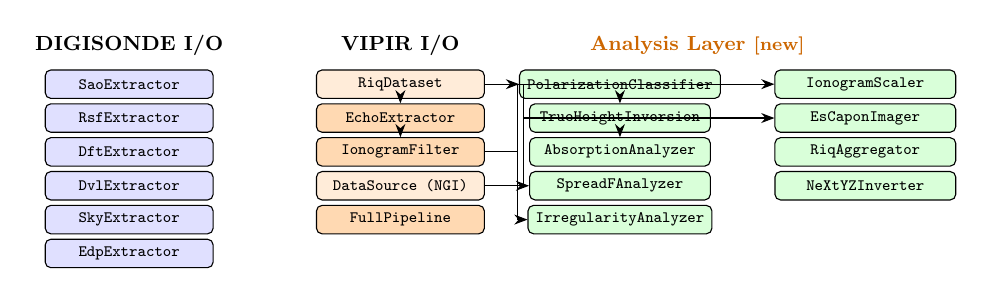
\begin{tikzpicture}[
  >=Stealth,
  every node/.style={font=\scriptsize},
  ioD/.style={draw,fill=blue!12,rounded corners=2pt,
              minimum width=2.6cm,minimum height=0.44cm,align=center},
  ioV/.style={draw,fill=orange!15,rounded corners=2pt,
              minimum width=2.6cm,minimum height=0.44cm,align=center},
  newV/.style={draw,fill=orange!30,rounded corners=2pt,
               minimum width=2.6cm,minimum height=0.44cm,align=center},
  an/.style={draw,fill=green!15,rounded corners=2pt,
             minimum width=2.8cm,minimum height=0.44cm,align=center},
  hdr/.style={font=\bfseries\small},
  scale=0.82,transform shape
]

\node[hdr] at (-4.2,2.4) {DIGISONDE I/O};
\node[hdr] at ( 0.0,2.4) {VIPIR I/O};
\node[hdr,text=orange!80!black] at ( 4.6,2.4) {Analysis Layer {\footnotesize[new]}};

%% DIGISONDE I/O column
\node[ioD] (sao)  at (-4.2, 1.8) {\texttt{SaoExtractor}};
\node[ioD,below=2pt of sao]  (rsf) {\texttt{RsfExtractor}};
\node[ioD,below=2pt of rsf]  (dft) {\texttt{DftExtractor}};
\node[ioD,below=2pt of dft]  (dvl) {\texttt{DvlExtractor}};
\node[ioD,below=2pt of dvl]  (sky) {\texttt{SkyExtractor}};
\node[ioD,below=2pt of sky]  (edp) {\texttt{EdpExtractor}};

%% VIPIR I/O column
\node[ioV] (riq)  at (0.0, 1.8)  {\texttt{RiqDataset}};
\node[newV,below=2pt of riq]  (echo) {\texttt{EchoExtractor}};
\node[newV,below=2pt of echo] (filt) {\texttt{IonogramFilter}};
\node[ioV,below=2pt of filt]  (ngi)  {\texttt{DataSource (NGI)}};
\node[newV,below=2pt of ngi]  (pipe) {\texttt{FullPipeline}};

%% Analysis layer — sub-column A
\node[an] (pol)  at (3.4, 1.8)  {\texttt{PolarizationClassifier}};
\node[an,below=2pt of pol]  (inv)  {\texttt{TrueHeightInversion}};
\node[an,below=2pt of inv]  (abs)  {\texttt{AbsorptionAnalyzer}};
\node[an,below=2pt of abs]  (sf)   {\texttt{SpreadFAnalyzer}};
\node[an,below=2pt of sf]   (irr)  {\texttt{IrregularityAnalyzer}};

%% Analysis layer — sub-column B
\node[an] (scl) at (7.2, 1.8)  {\texttt{IonogramScaler}};
\node[an,below=2pt of scl]  (es)   {\texttt{EsCaponImager}};
\node[an,below=2pt of es]   (agg)  {\texttt{RiqAggregator}};
\node[an,below=2pt of agg]  (nxt)  {\texttt{NeXtYZInverter}};

%% Arrows
\draw[->] (riq.south)  -- (echo.north);
\draw[->] (echo.south) -- (filt.north);
\draw[->] (filt.east)  -- ++(0.5,0) |- (pol.west);
\draw[->] (filt.east)  -- ++(0.5,0) |- (sf.west);
\draw[->] (filt.east)  -- ++(0.5,0) |- (irr.west);
\draw[->] (pol.south)  -- (inv.north);
\draw[->] (inv.south)  -- (abs.north);
\draw[->] (riq.east)   -- ++(0.6,0) |- (es.west);
\draw[->] (ngi.east)   -- ++(0.6,0) |- (scl.west);

\end{tikzpicture}
\end{center}
\vspace{0.1cm}
{\scriptsize Orange = new since v1.0 publication.\ \ Green = analysis layer (entirely post-v1.0).}
\end{frame}

% ----------------------------------------------------------------
\section{Installation \& Quick Start}
% ----------------------------------------------------------------

\begin{frame}[fragile]{Installation}
  \begin{lstlisting}[title={Terminal}]
# Option 1: PyPI
pip install pynasonde

# Option 2: developer install (recommended for this workshop)
git clone https://github.com/shibaji7/pynasonde.git
cd pynasonde
pip install -e ".[dev]"
  \end{lstlisting}

  \begin{block}{Requirements}
    Python $\ge$ 3.11 \quad|\quad
    numpy, pandas, scipy, matplotlib, loguru
  \end{block}
\end{frame}

% ----------------------------------------------------------------
\section{DIGISONDE Data}
% ----------------------------------------------------------------

\begin{frame}[fragile]{SAO — Electron Density Profiles}
  The \texttt{.SAO} file contains scaled ionogram parameters and height profiles:
  \begin{lstlisting}
from pynasonde.digisonde.parsers.sao import SaoExtractor

# Load a day of SAO files in parallel (n_procs workers)
df = SaoExtractor.load_SAO_files(
    folders=["data/KR835/"],
    func_name="height_profile",
    n_procs=4,
)
print(df.columns.tolist())
# ['datetime', 'height_km', 'plasma_freq_mhz', 'electron_density_cm3', ...]
  \end{lstlisting}
  \begin{itemize}\small
    \item \texttt{func\_name="height\_profile"} — N(h) profile per record
    \item \texttt{func\_name="scaled\_params"} — foF2, hmF2, MUF, foE
  \end{itemize}
\end{frame}

\begin{frame}{SAO — Isodensity Contour Plot}
  \begin{center}
    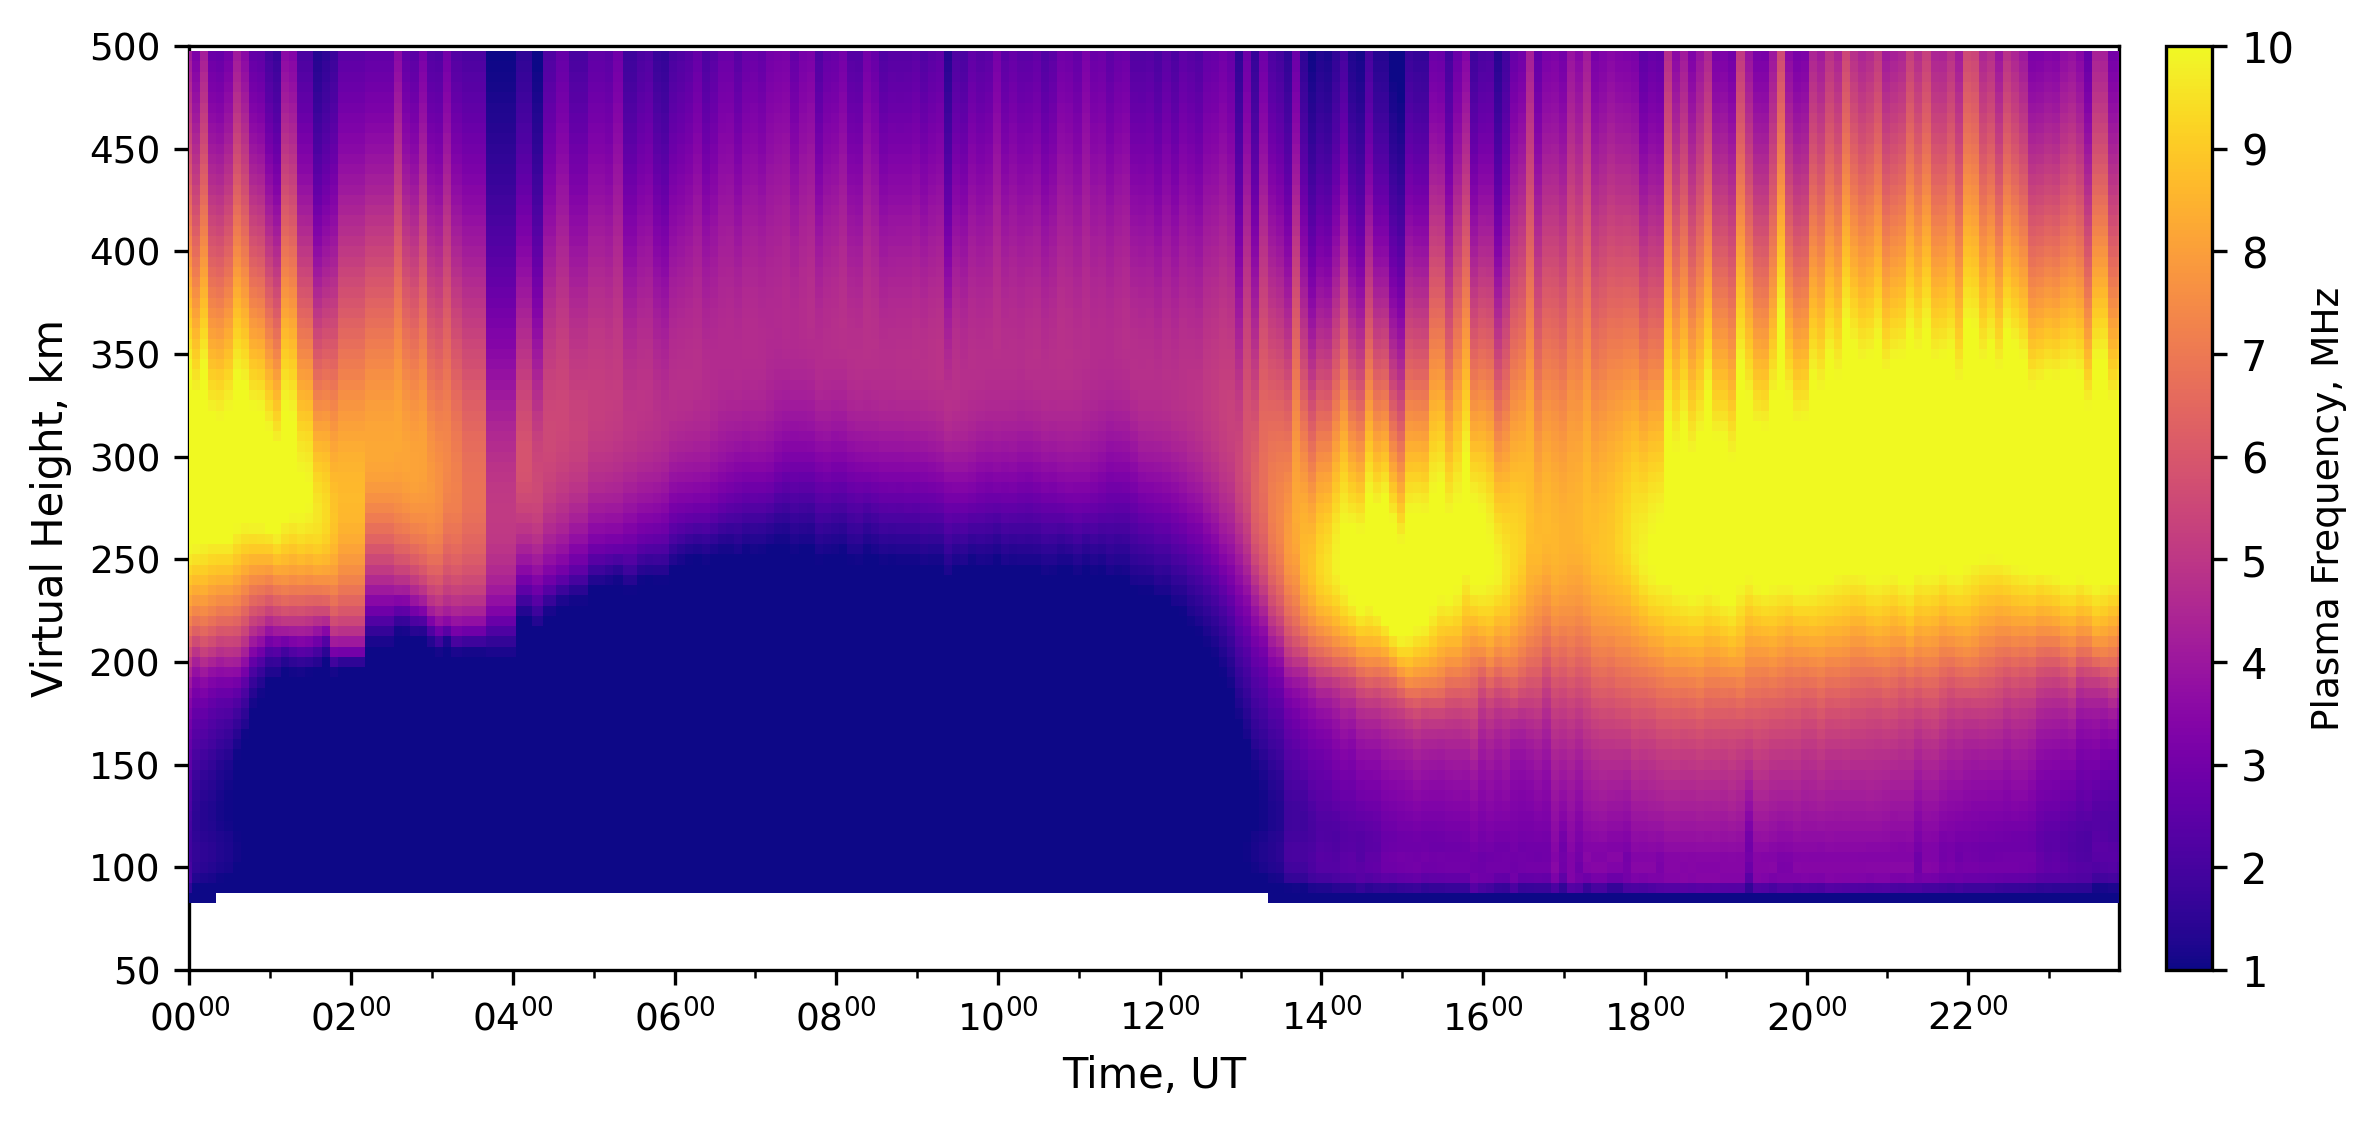
\includegraphics[width=0.82\linewidth]{sao_isodensity_KR835.png}
  \end{center}
  \vspace{-0.3cm}
  {\small Daily isodensity contour from DPS4D SAO files at KR835.
  Each horizontal slice is one N(h) profile; colour encodes electron density.}
\end{frame}

\begin{frame}{SAO — N(h) Profile and F2 Parameters}
  \begin{columns}
  \column{0.48\textwidth}
    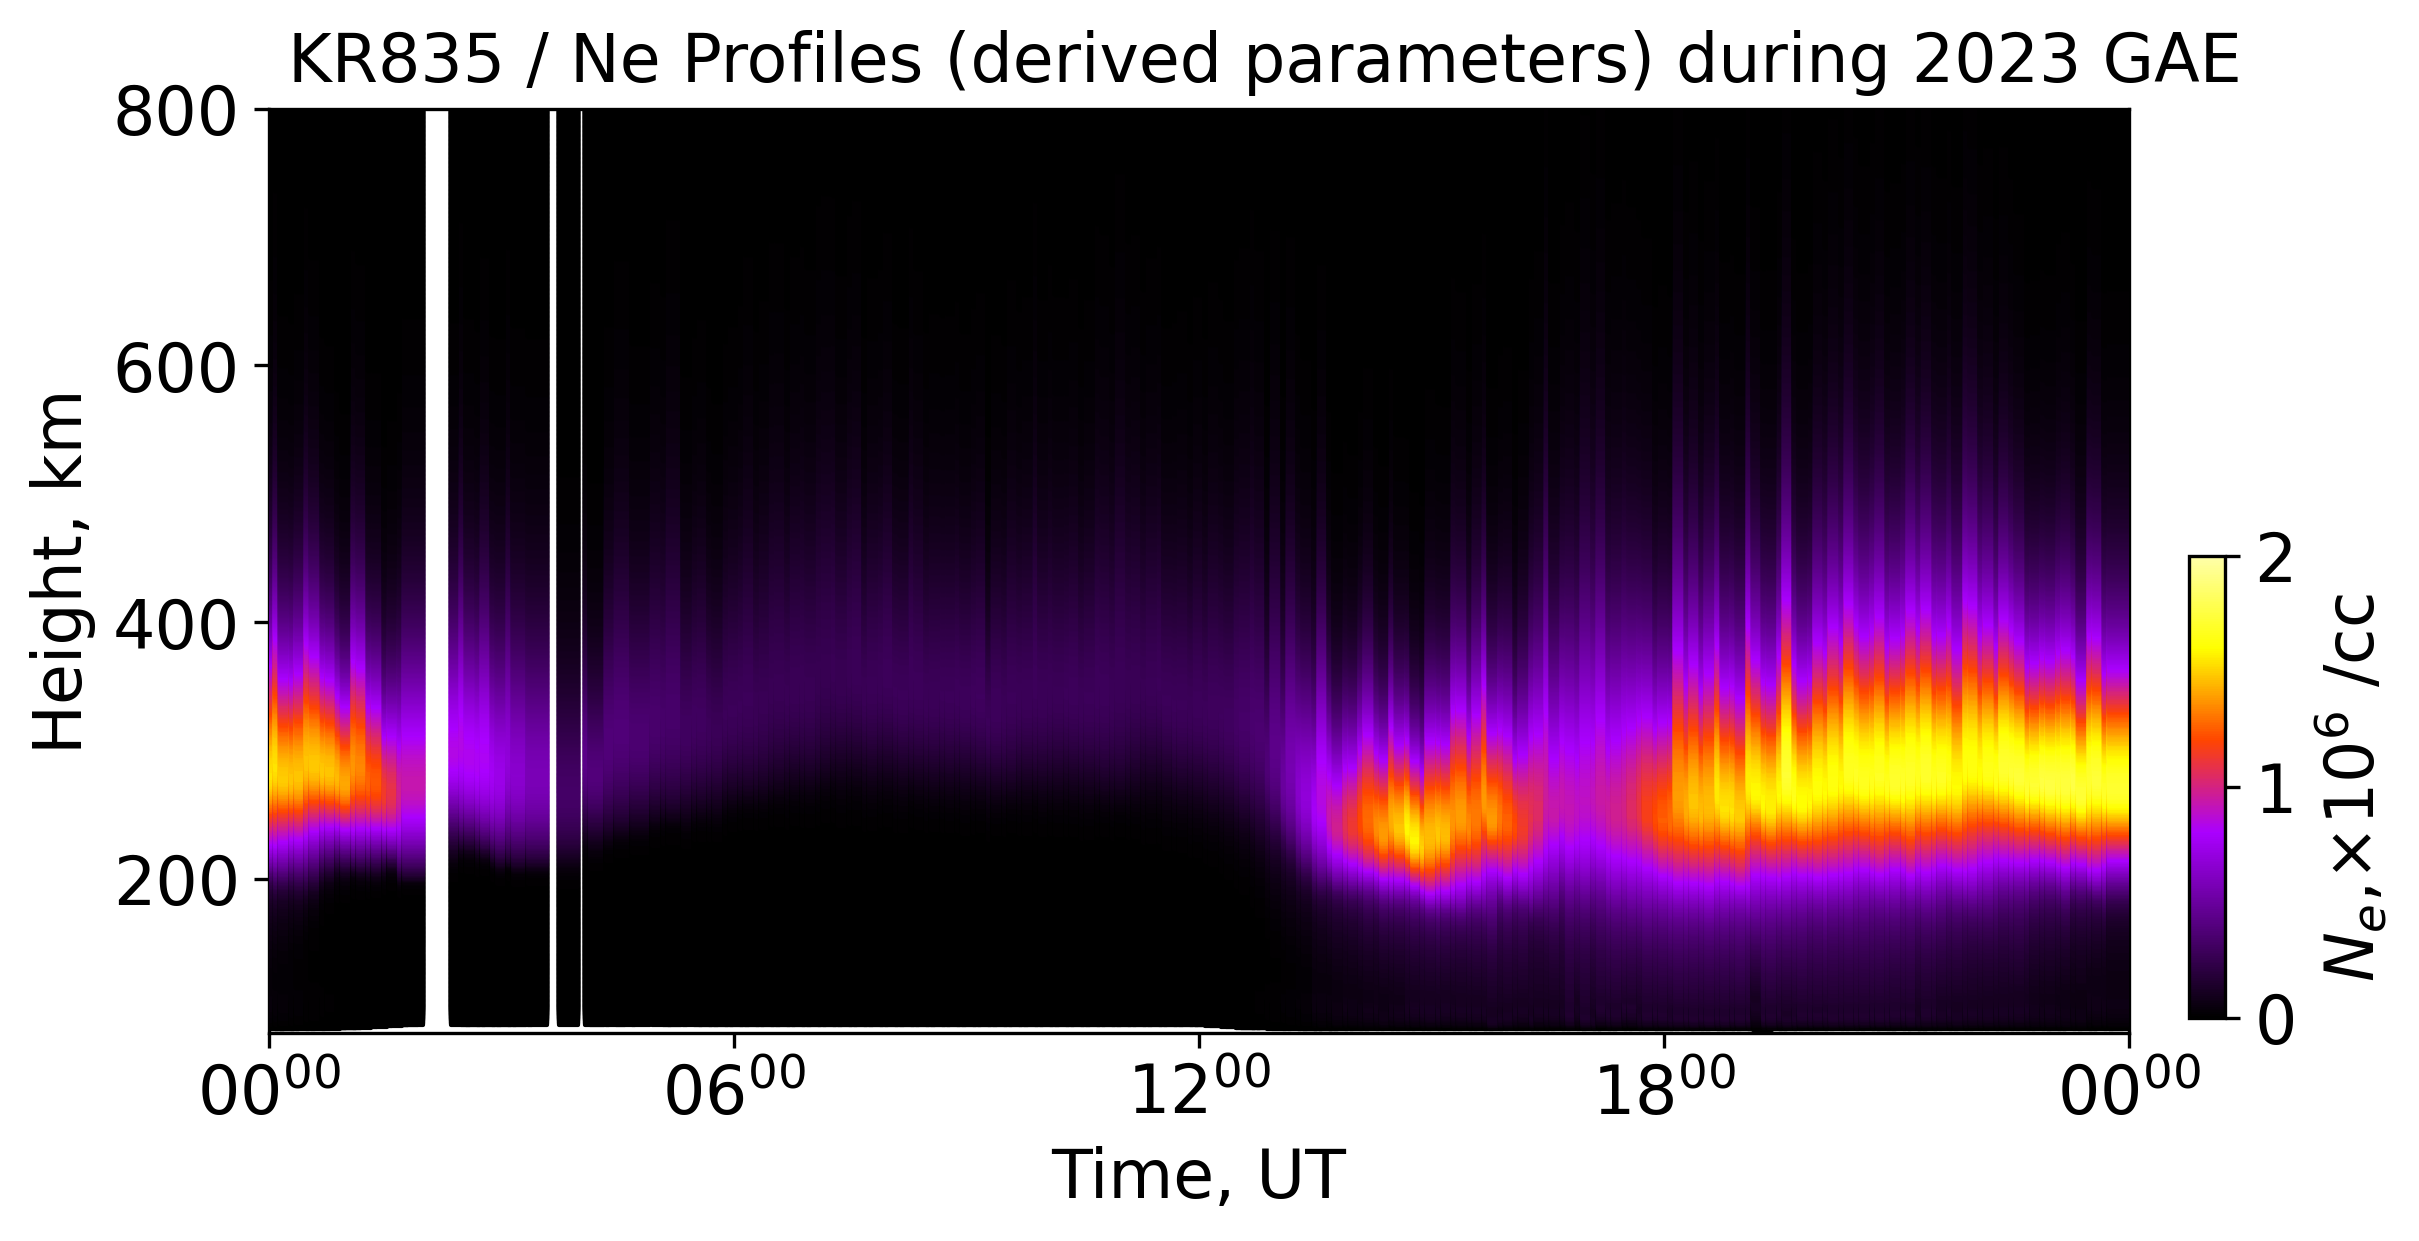
\includegraphics[width=\linewidth,height=3.8cm,keepaspectratio]{stack_sao_ne.png}
  \column{0.48\textwidth}
    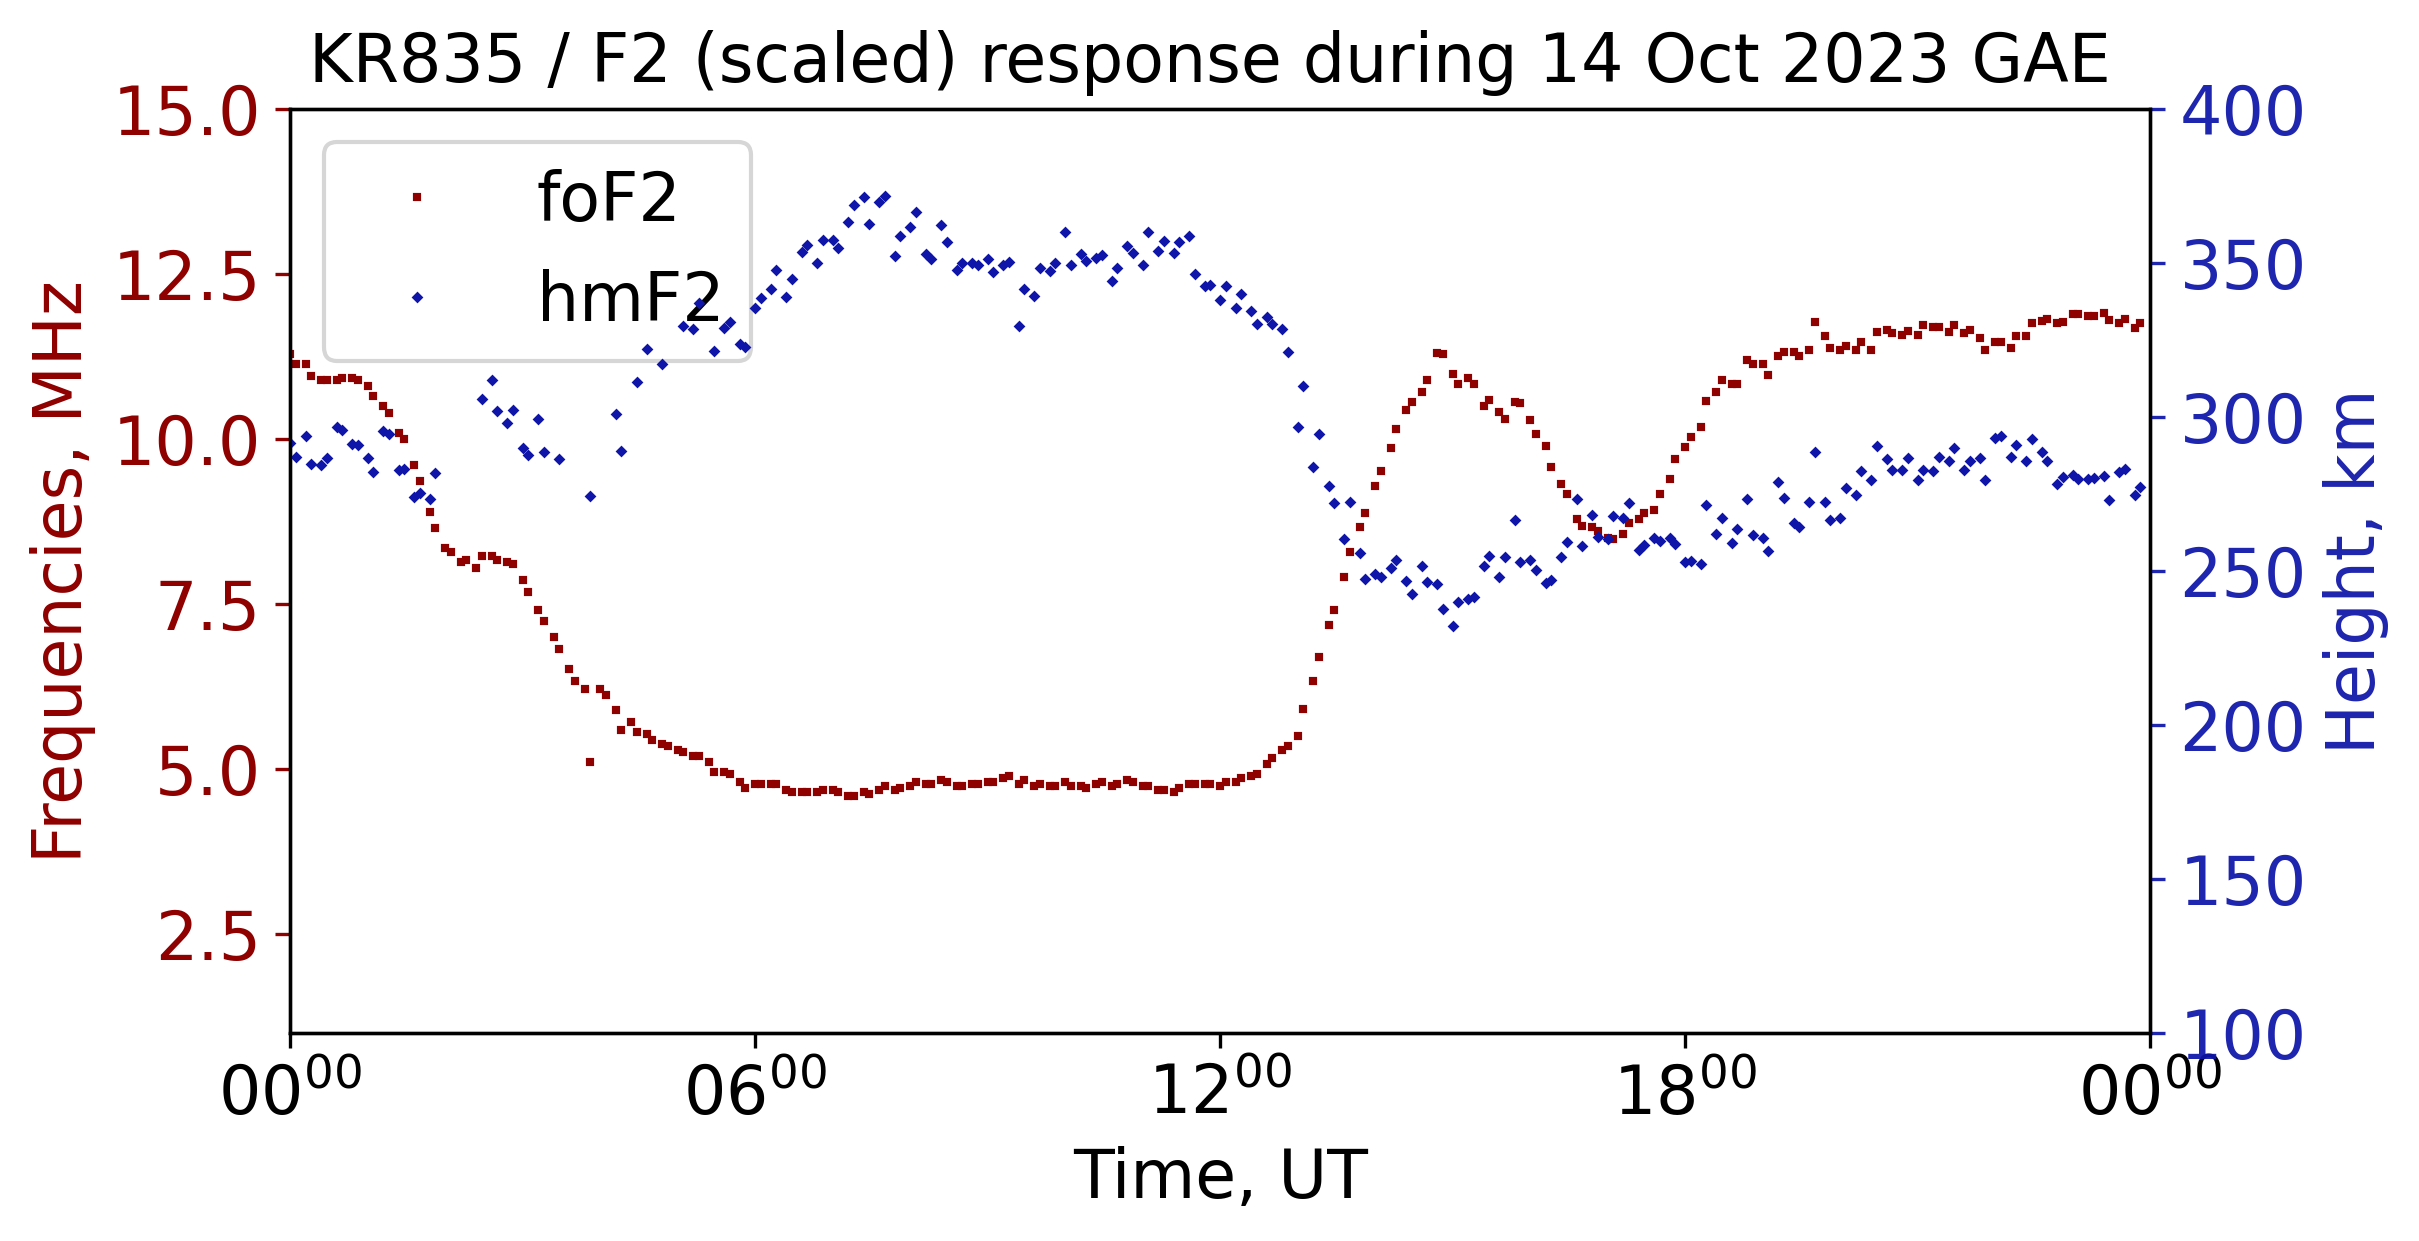
\includegraphics[width=\linewidth,height=3.8cm,keepaspectratio]{stack_sao_F2.png}
  \end{columns}
  {\small Left: stacked N(h) profiles. Right: daily foF2 and hmF2 time series.}
\end{frame}

\begin{frame}[fragile]{RSF — Direction-Coded Ionogram}
  \texttt{.RSF} files store raw amplitude+phase for each sounding:
  \begin{lstlisting}
from pynasonde.digisonde.parsers.rsf import RsfExtractor

extractor = RsfExtractor("data/KR835_20230601.RSF")
extractor.extract()
df = extractor.to_dataframe()
extractor.plot_direction_ionogram()   # direction-coded ionogram
extractor.plot_directogram()          # full-day directogram
  \end{lstlisting}
\end{frame}

\begin{frame}{RSF — Direction-Coded Ionogram \& Directogram}
  \begin{columns}
  \column{0.50\textwidth}
    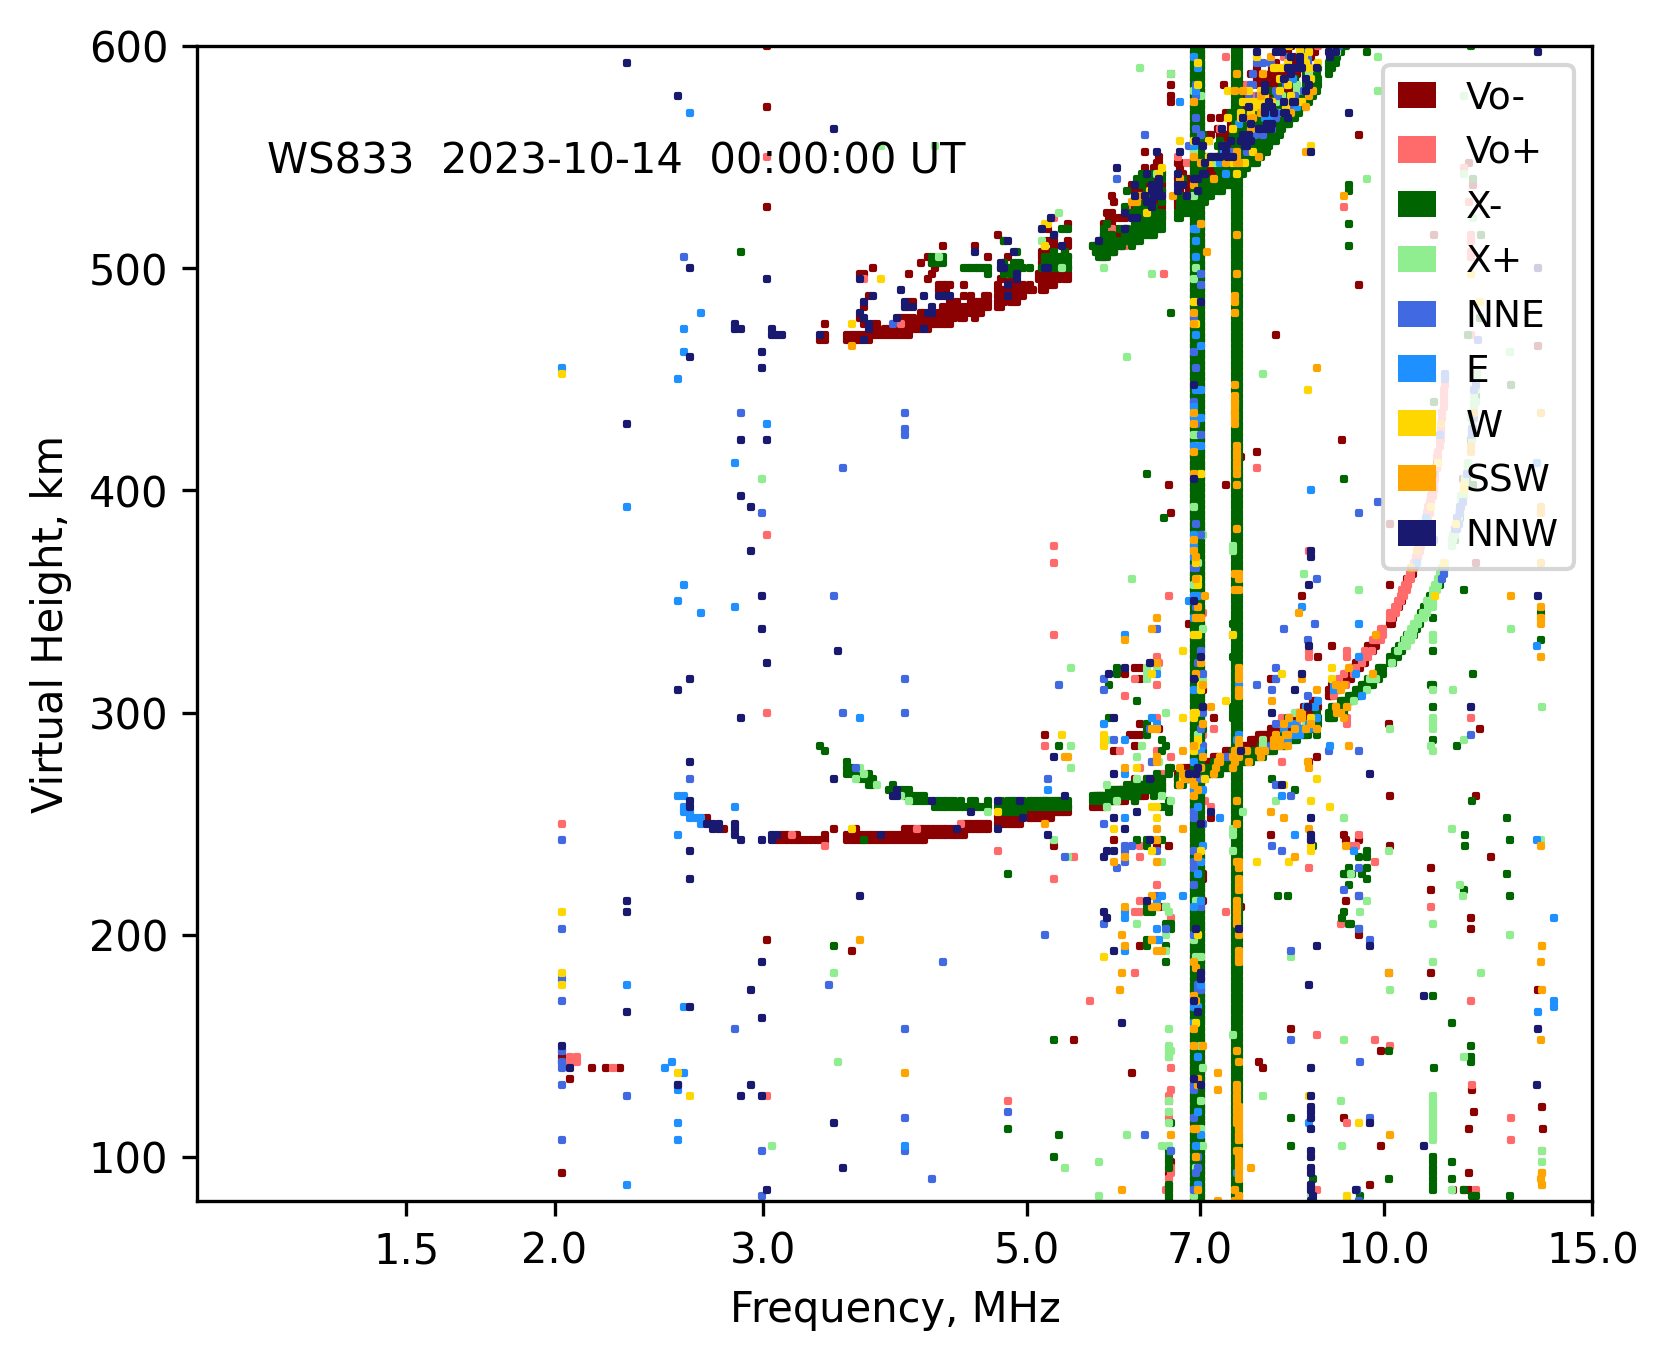
\includegraphics[width=\linewidth,height=3.8cm,keepaspectratio]{rsf_direction_ionogram_KR835.png}
  \column{0.46\textwidth}
    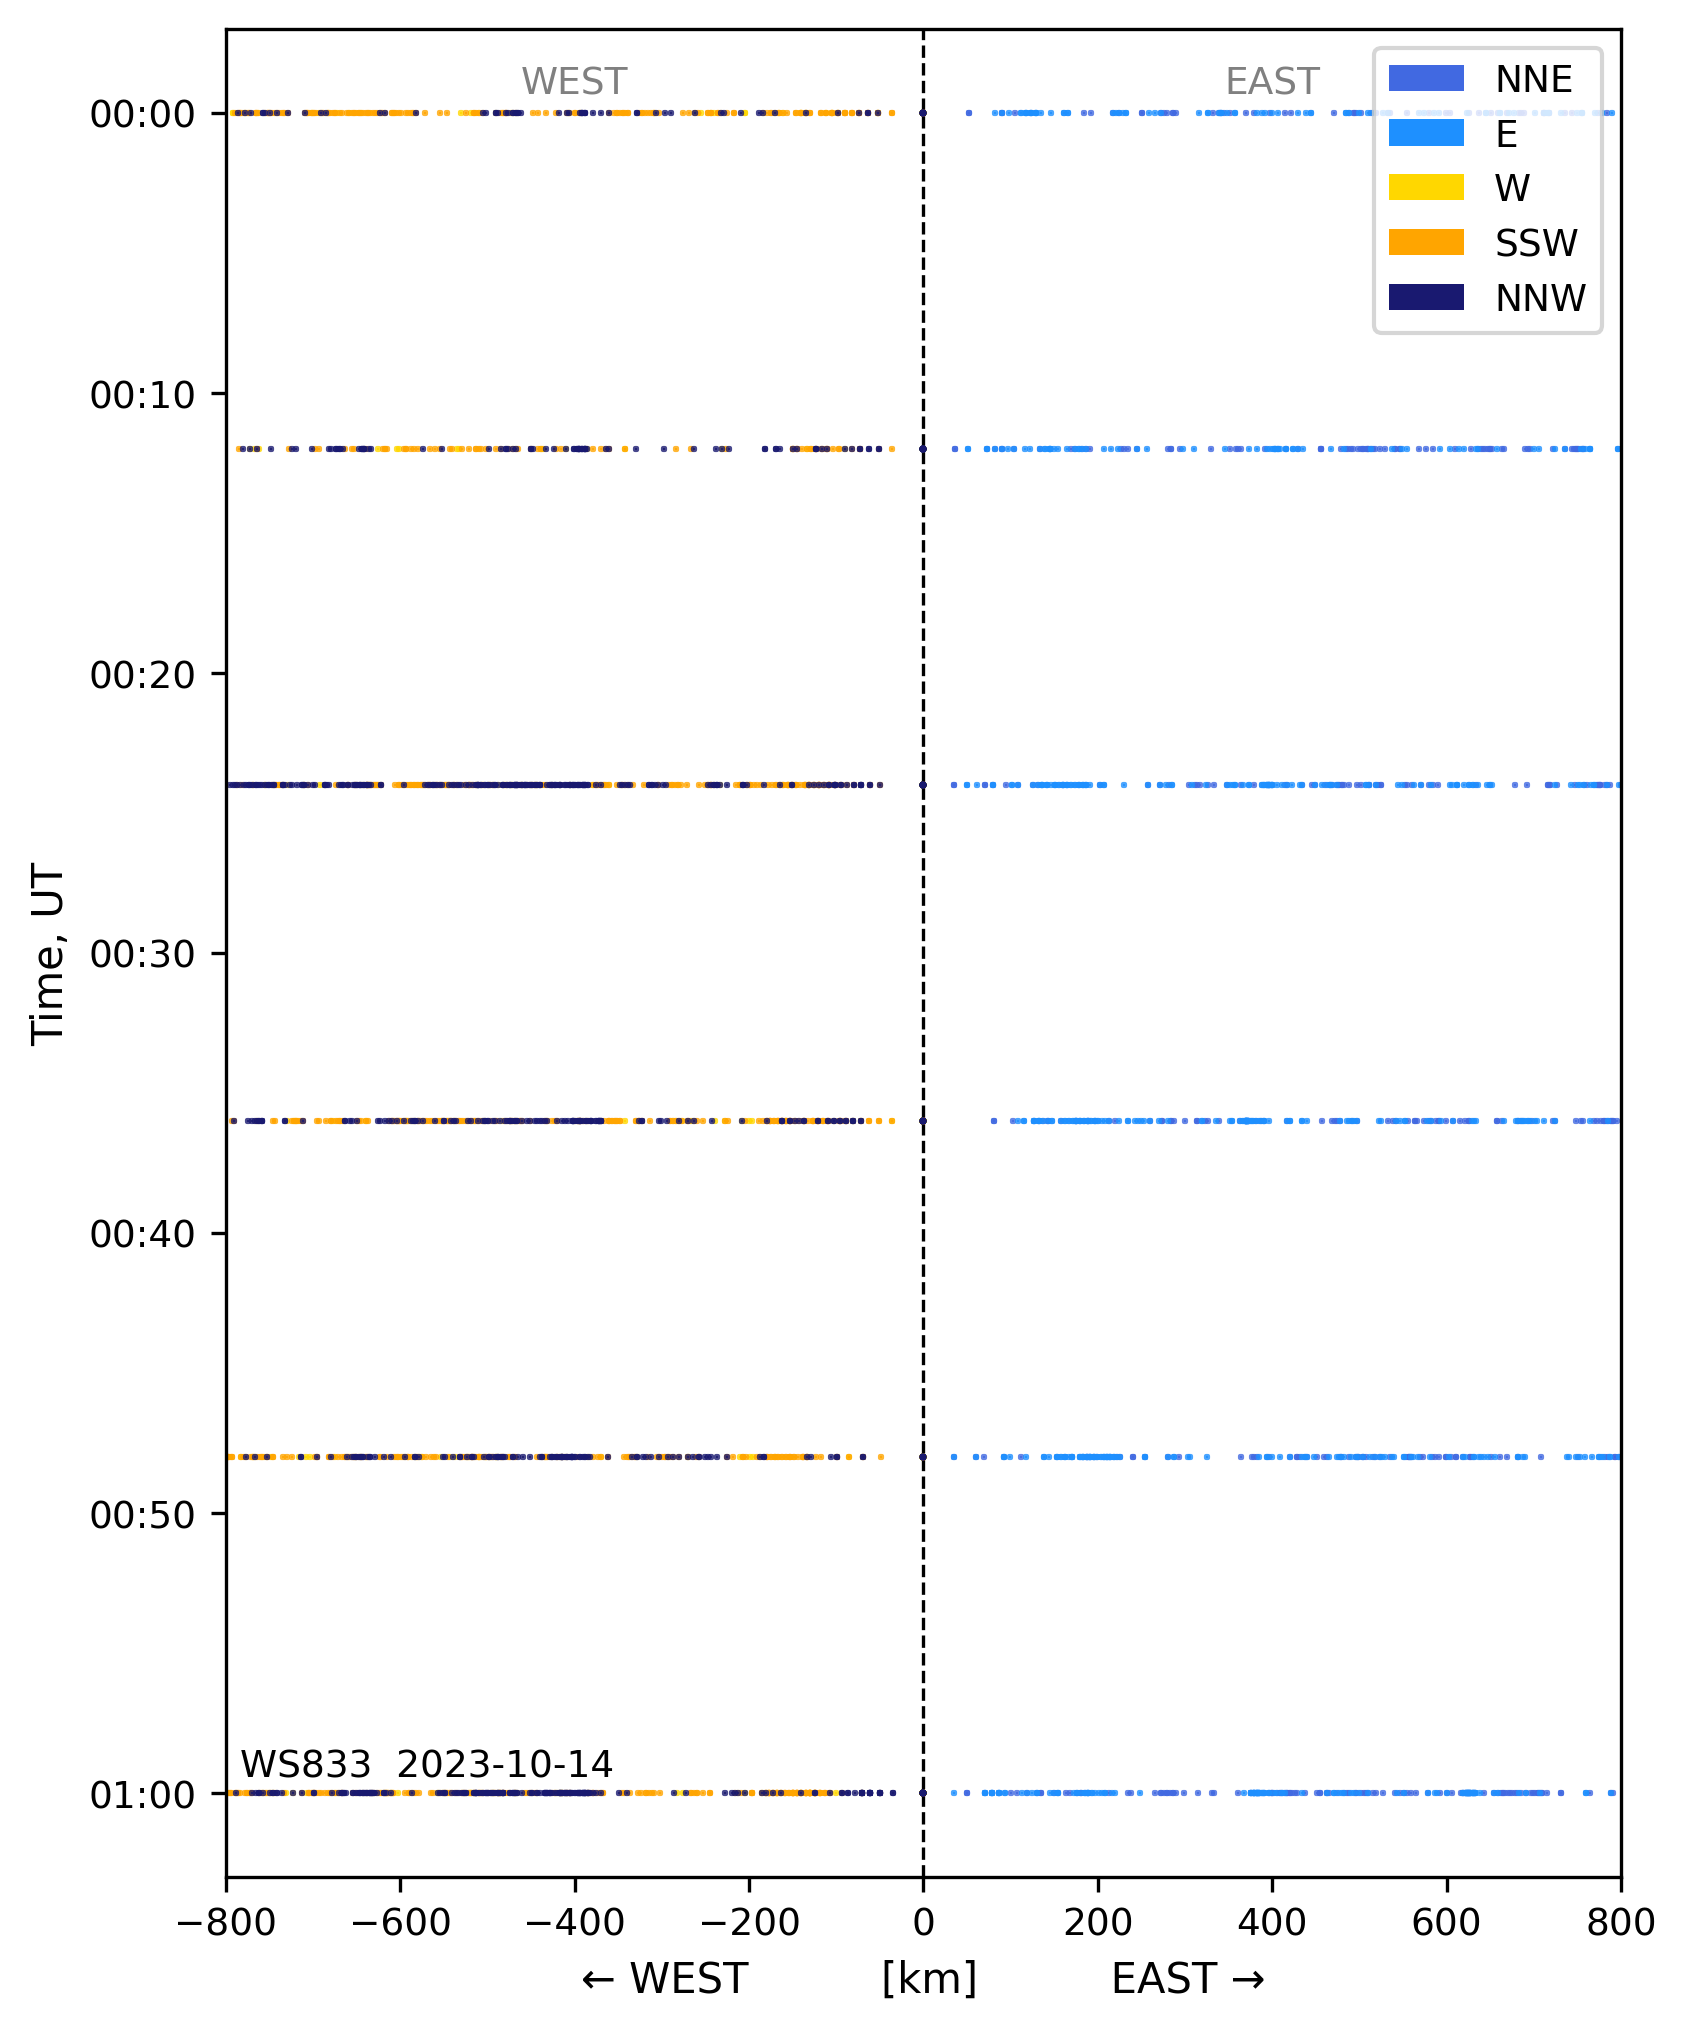
\includegraphics[width=\linewidth,height=3.8cm,keepaspectratio]{rsf_directogram_KR835_daily.png}
  \end{columns}
  {\small Left: direction-coded ionogram (colour = arrival azimuth).
   Right: daily directogram (time vs.\ ground distance).}
\end{frame}

\begin{frame}[fragile]{DFT — Doppler Waterfall \& Spectra}
  \texttt{.DFT} files contain per-height Doppler spectra:
  \begin{lstlisting}
from pynasonde.digisonde.parsers.dft import DftExtractor

dft = DftExtractor("data/KR835_20230601.DFT")
dft.extract()
dft.plot_doppler_waterfall()   # time-height Doppler waterfall
dft.plot_doppler_spectra()     # per-height spectra
  \end{lstlisting}
\end{frame}

\begin{frame}{DFT — Doppler Waterfall \& Spectra}
  \begin{columns}
  \column{0.50\textwidth}
    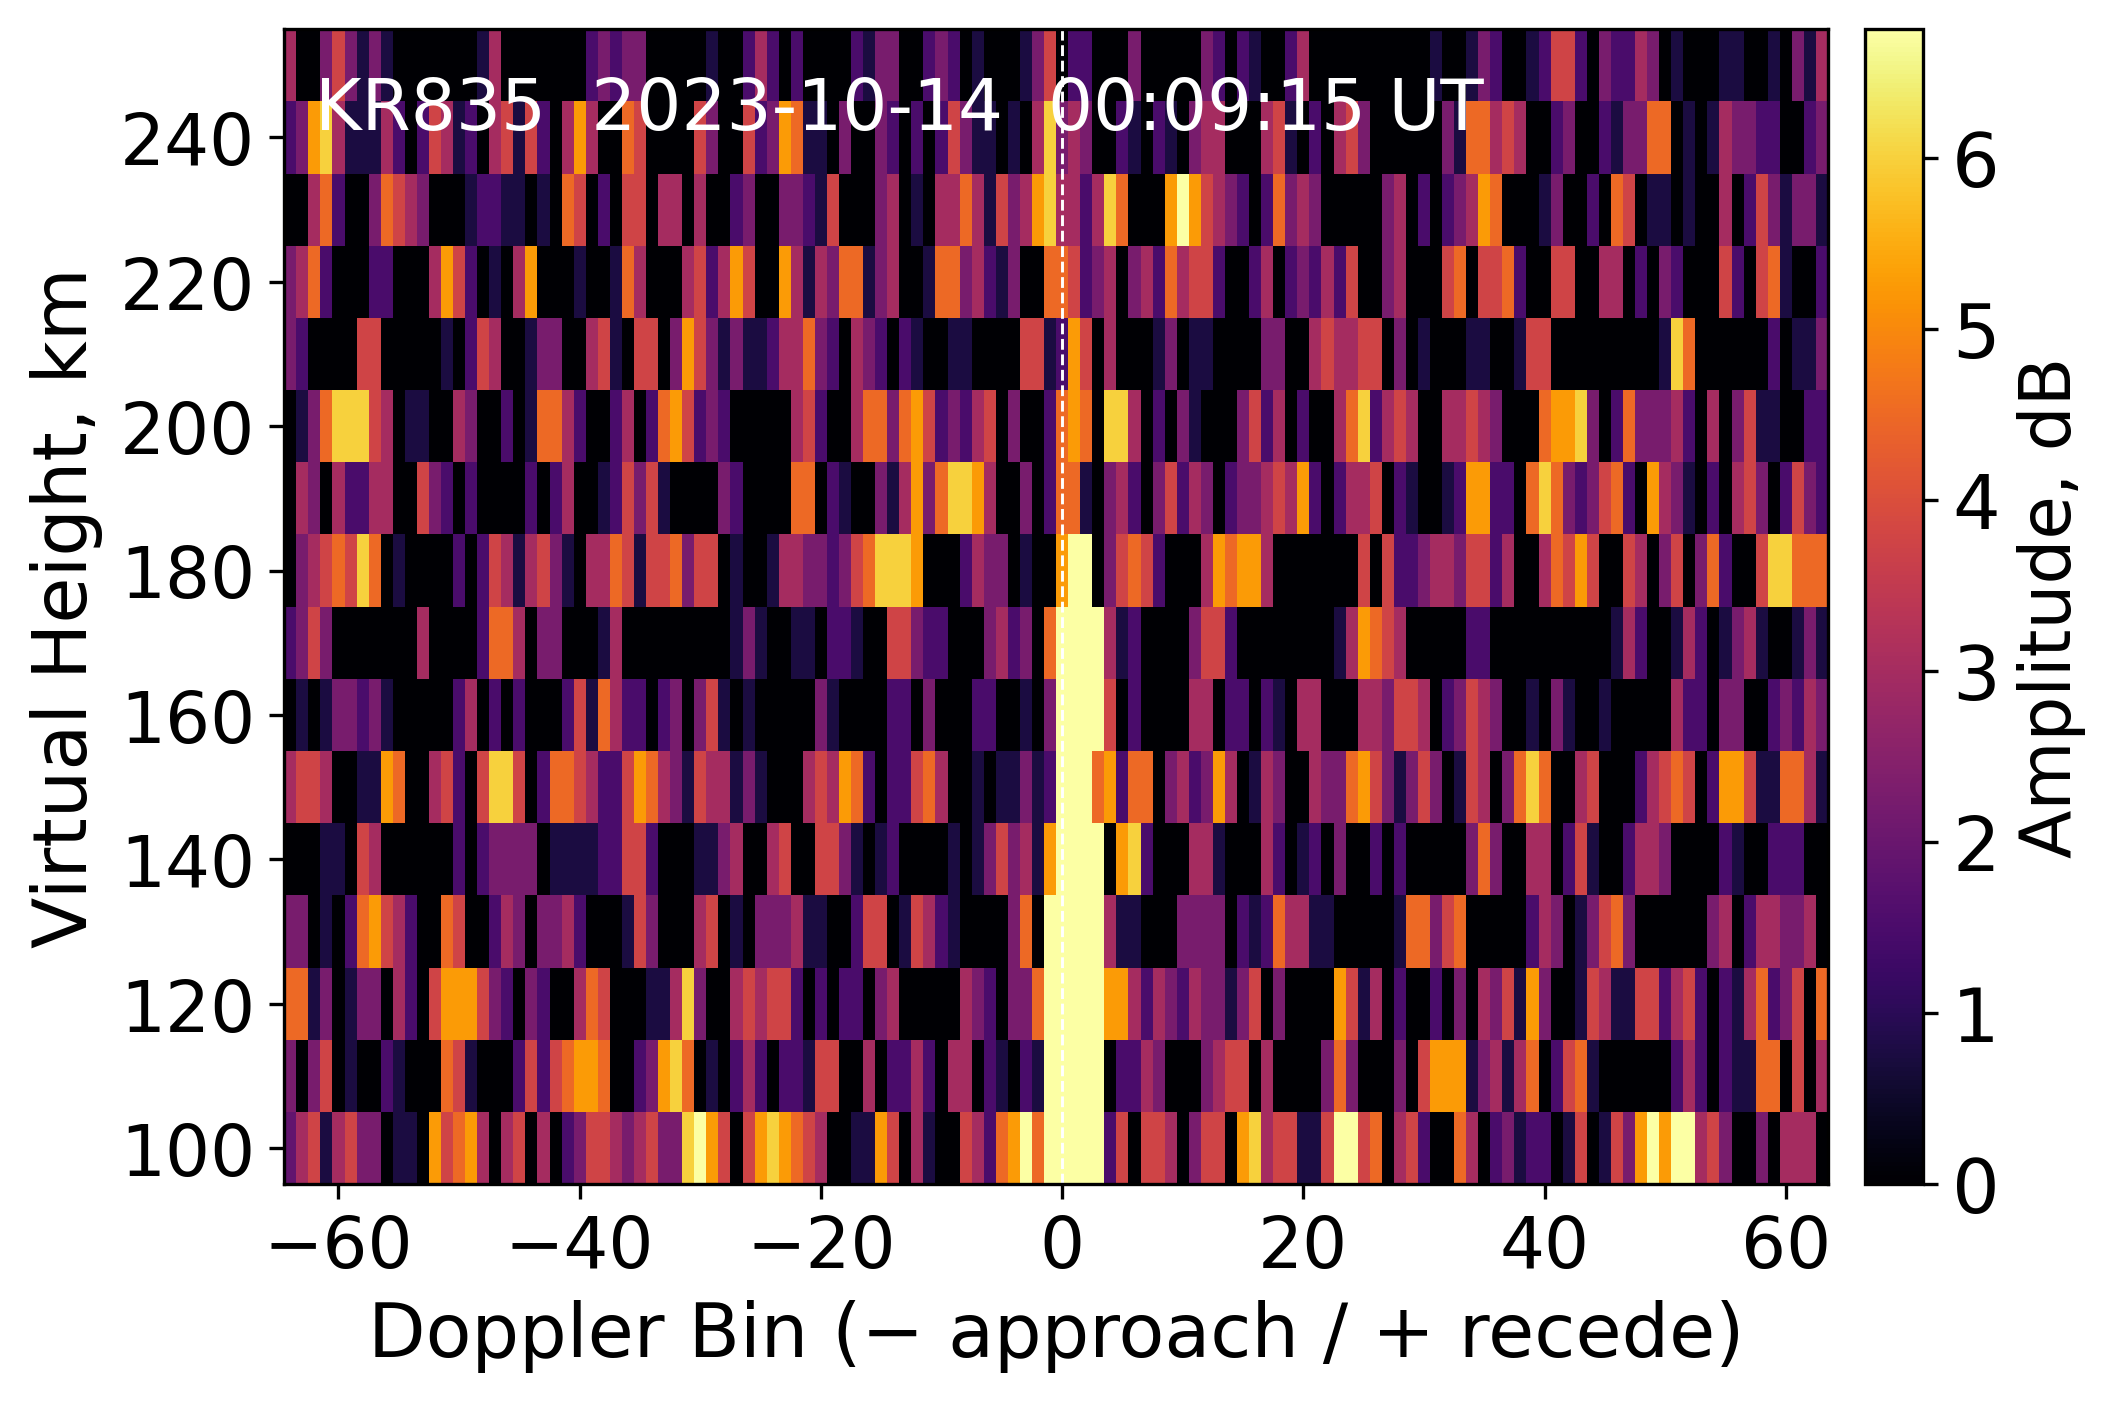
\includegraphics[width=\linewidth,height=3.8cm,keepaspectratio]{dft_doppler_waterfall_KR835.png}
  \column{0.46\textwidth}
    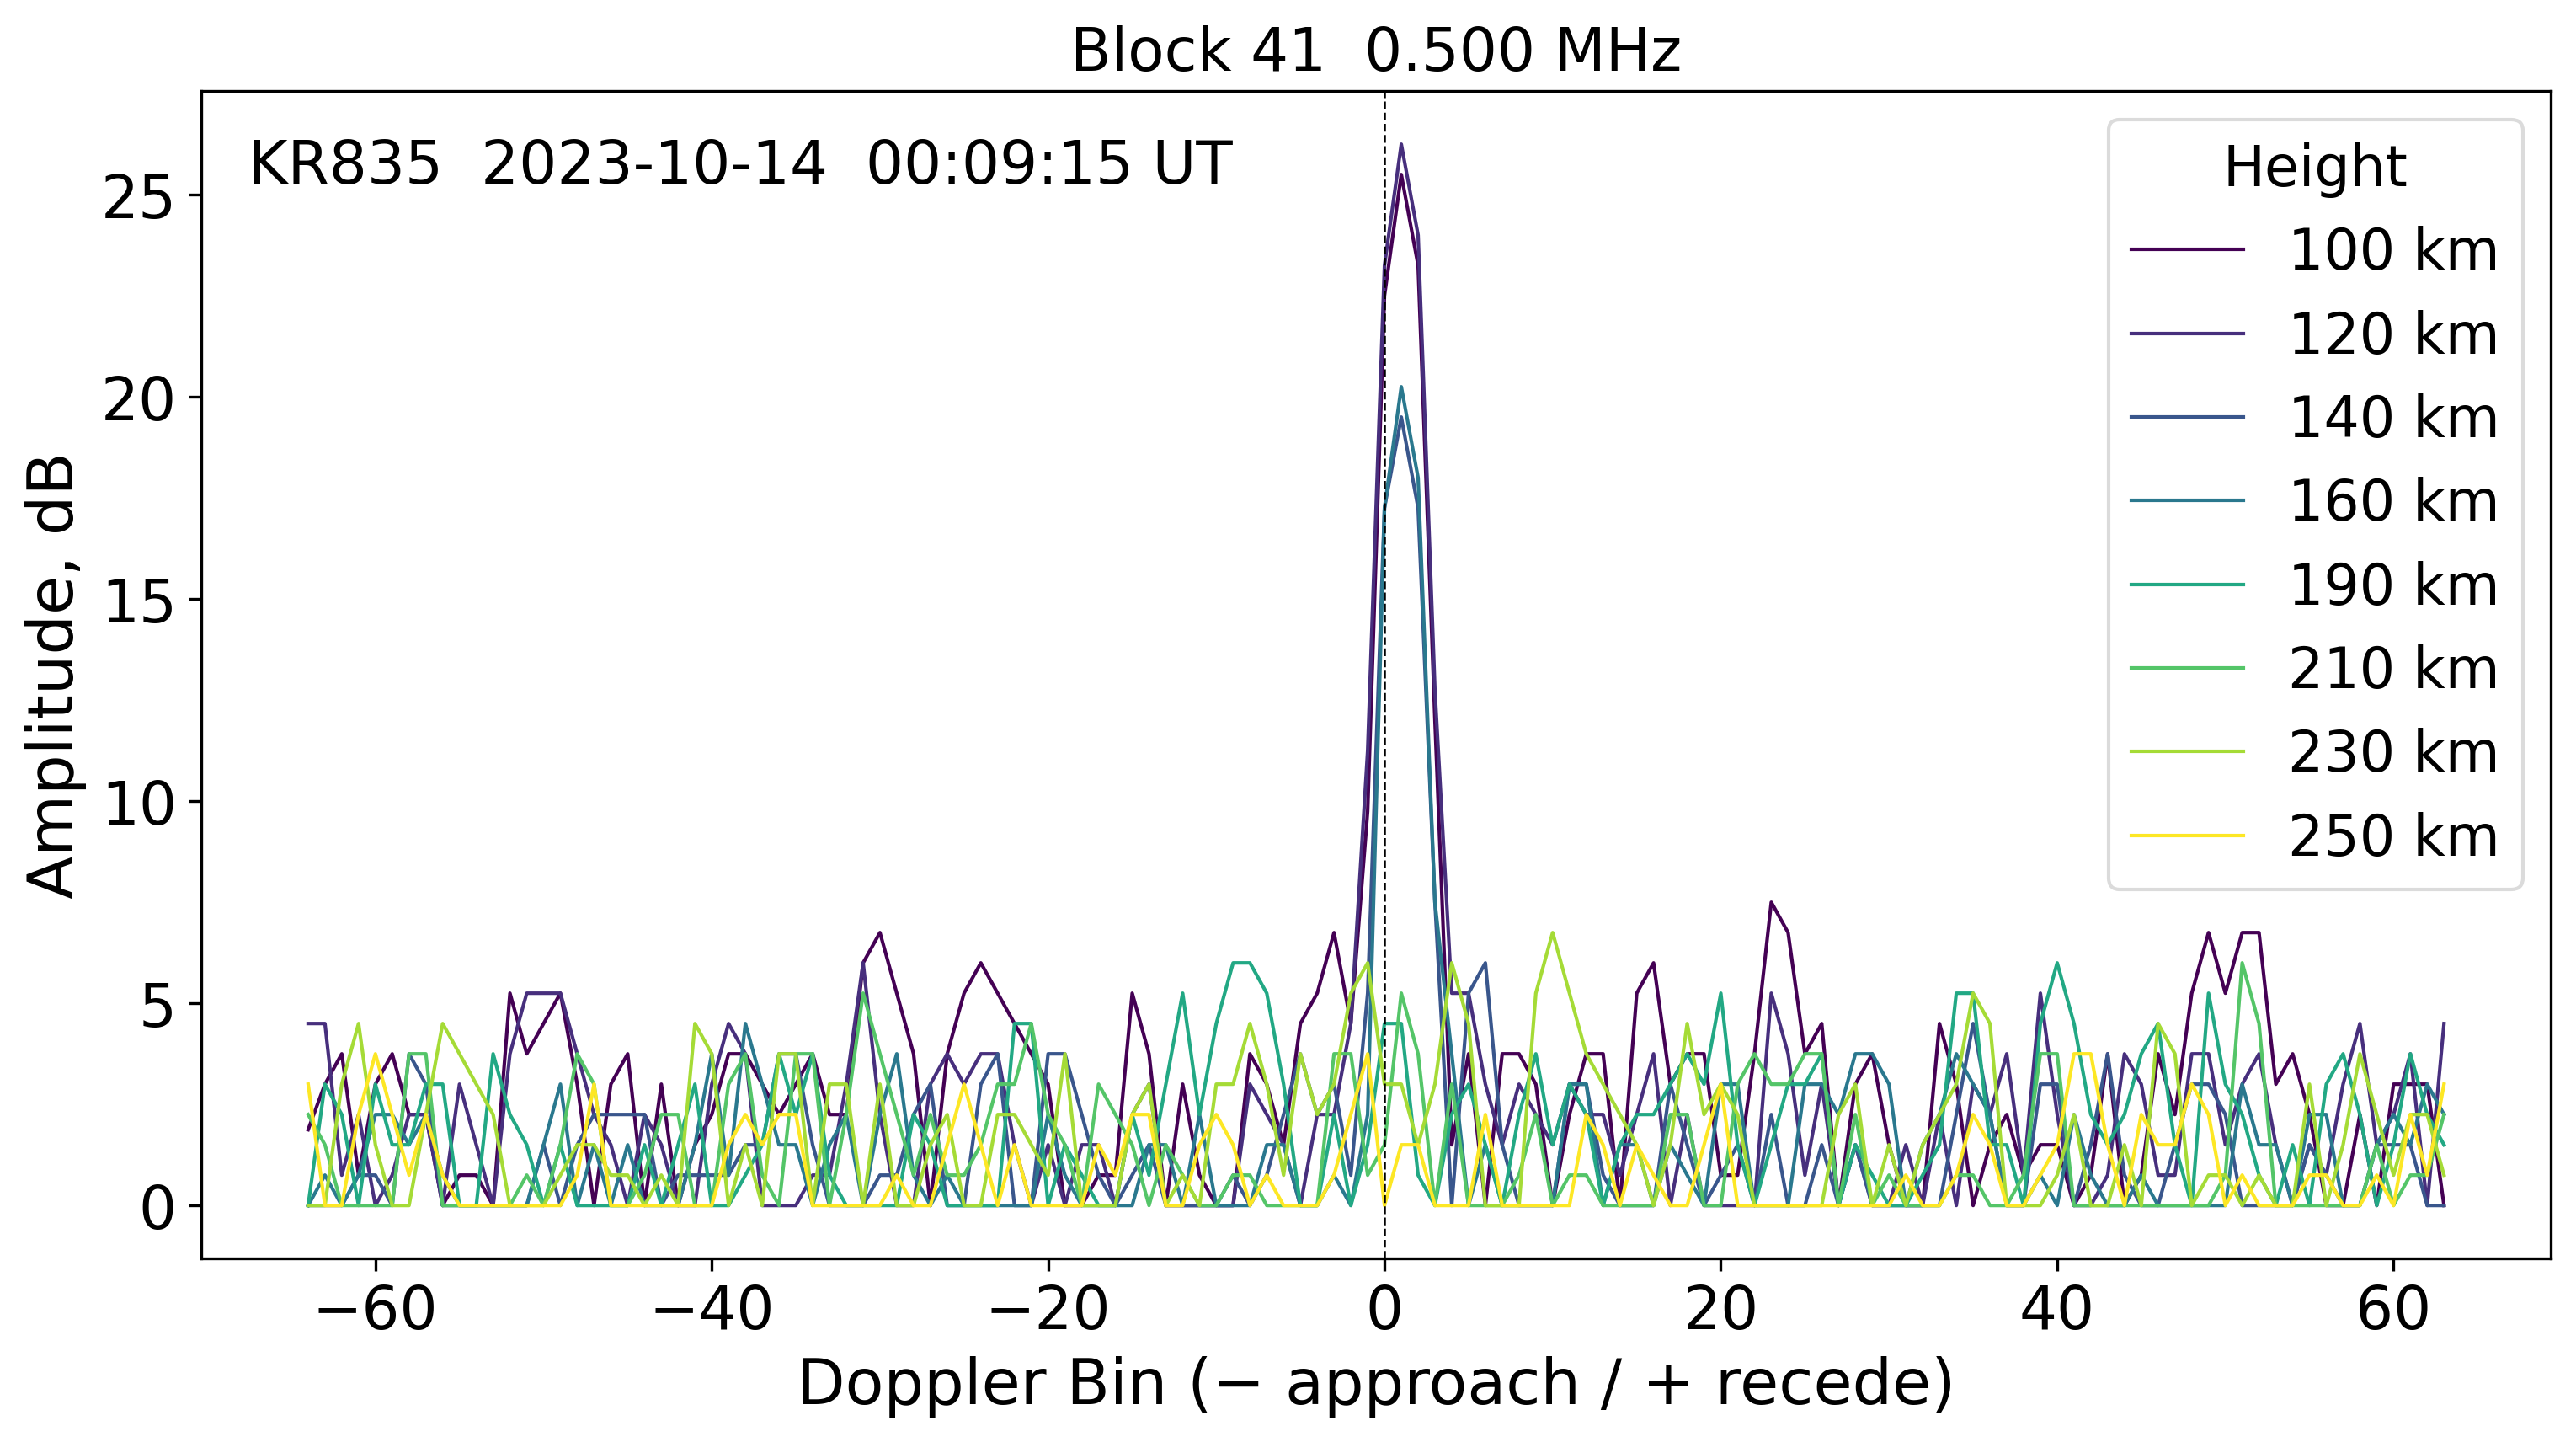
\includegraphics[width=\linewidth,height=3.8cm,keepaspectratio]{dft_doppler_spectra_KR835.png}
  \end{columns}
  {\small Left: Doppler velocity waterfall (height vs.\ time).
   Right: per-height Doppler spectra at one epoch.}
\end{frame}

\begin{frame}[fragile]{DVL — Drift Velocity Stack Plot}
  \texttt{.DVL} files contain the ionospheric drift velocity estimates:
  \begin{lstlisting}
from pynasonde.digisonde.parsers.dvl import DvlExtractor

dvl = DvlExtractor.load_files(folder="data/KR835/", n_procs=4)
dvl.plot_stack()   # 3-panel Vx, Vy, Vz vs. time + virtual height overlay
  \end{lstlisting}
  \begin{center}
    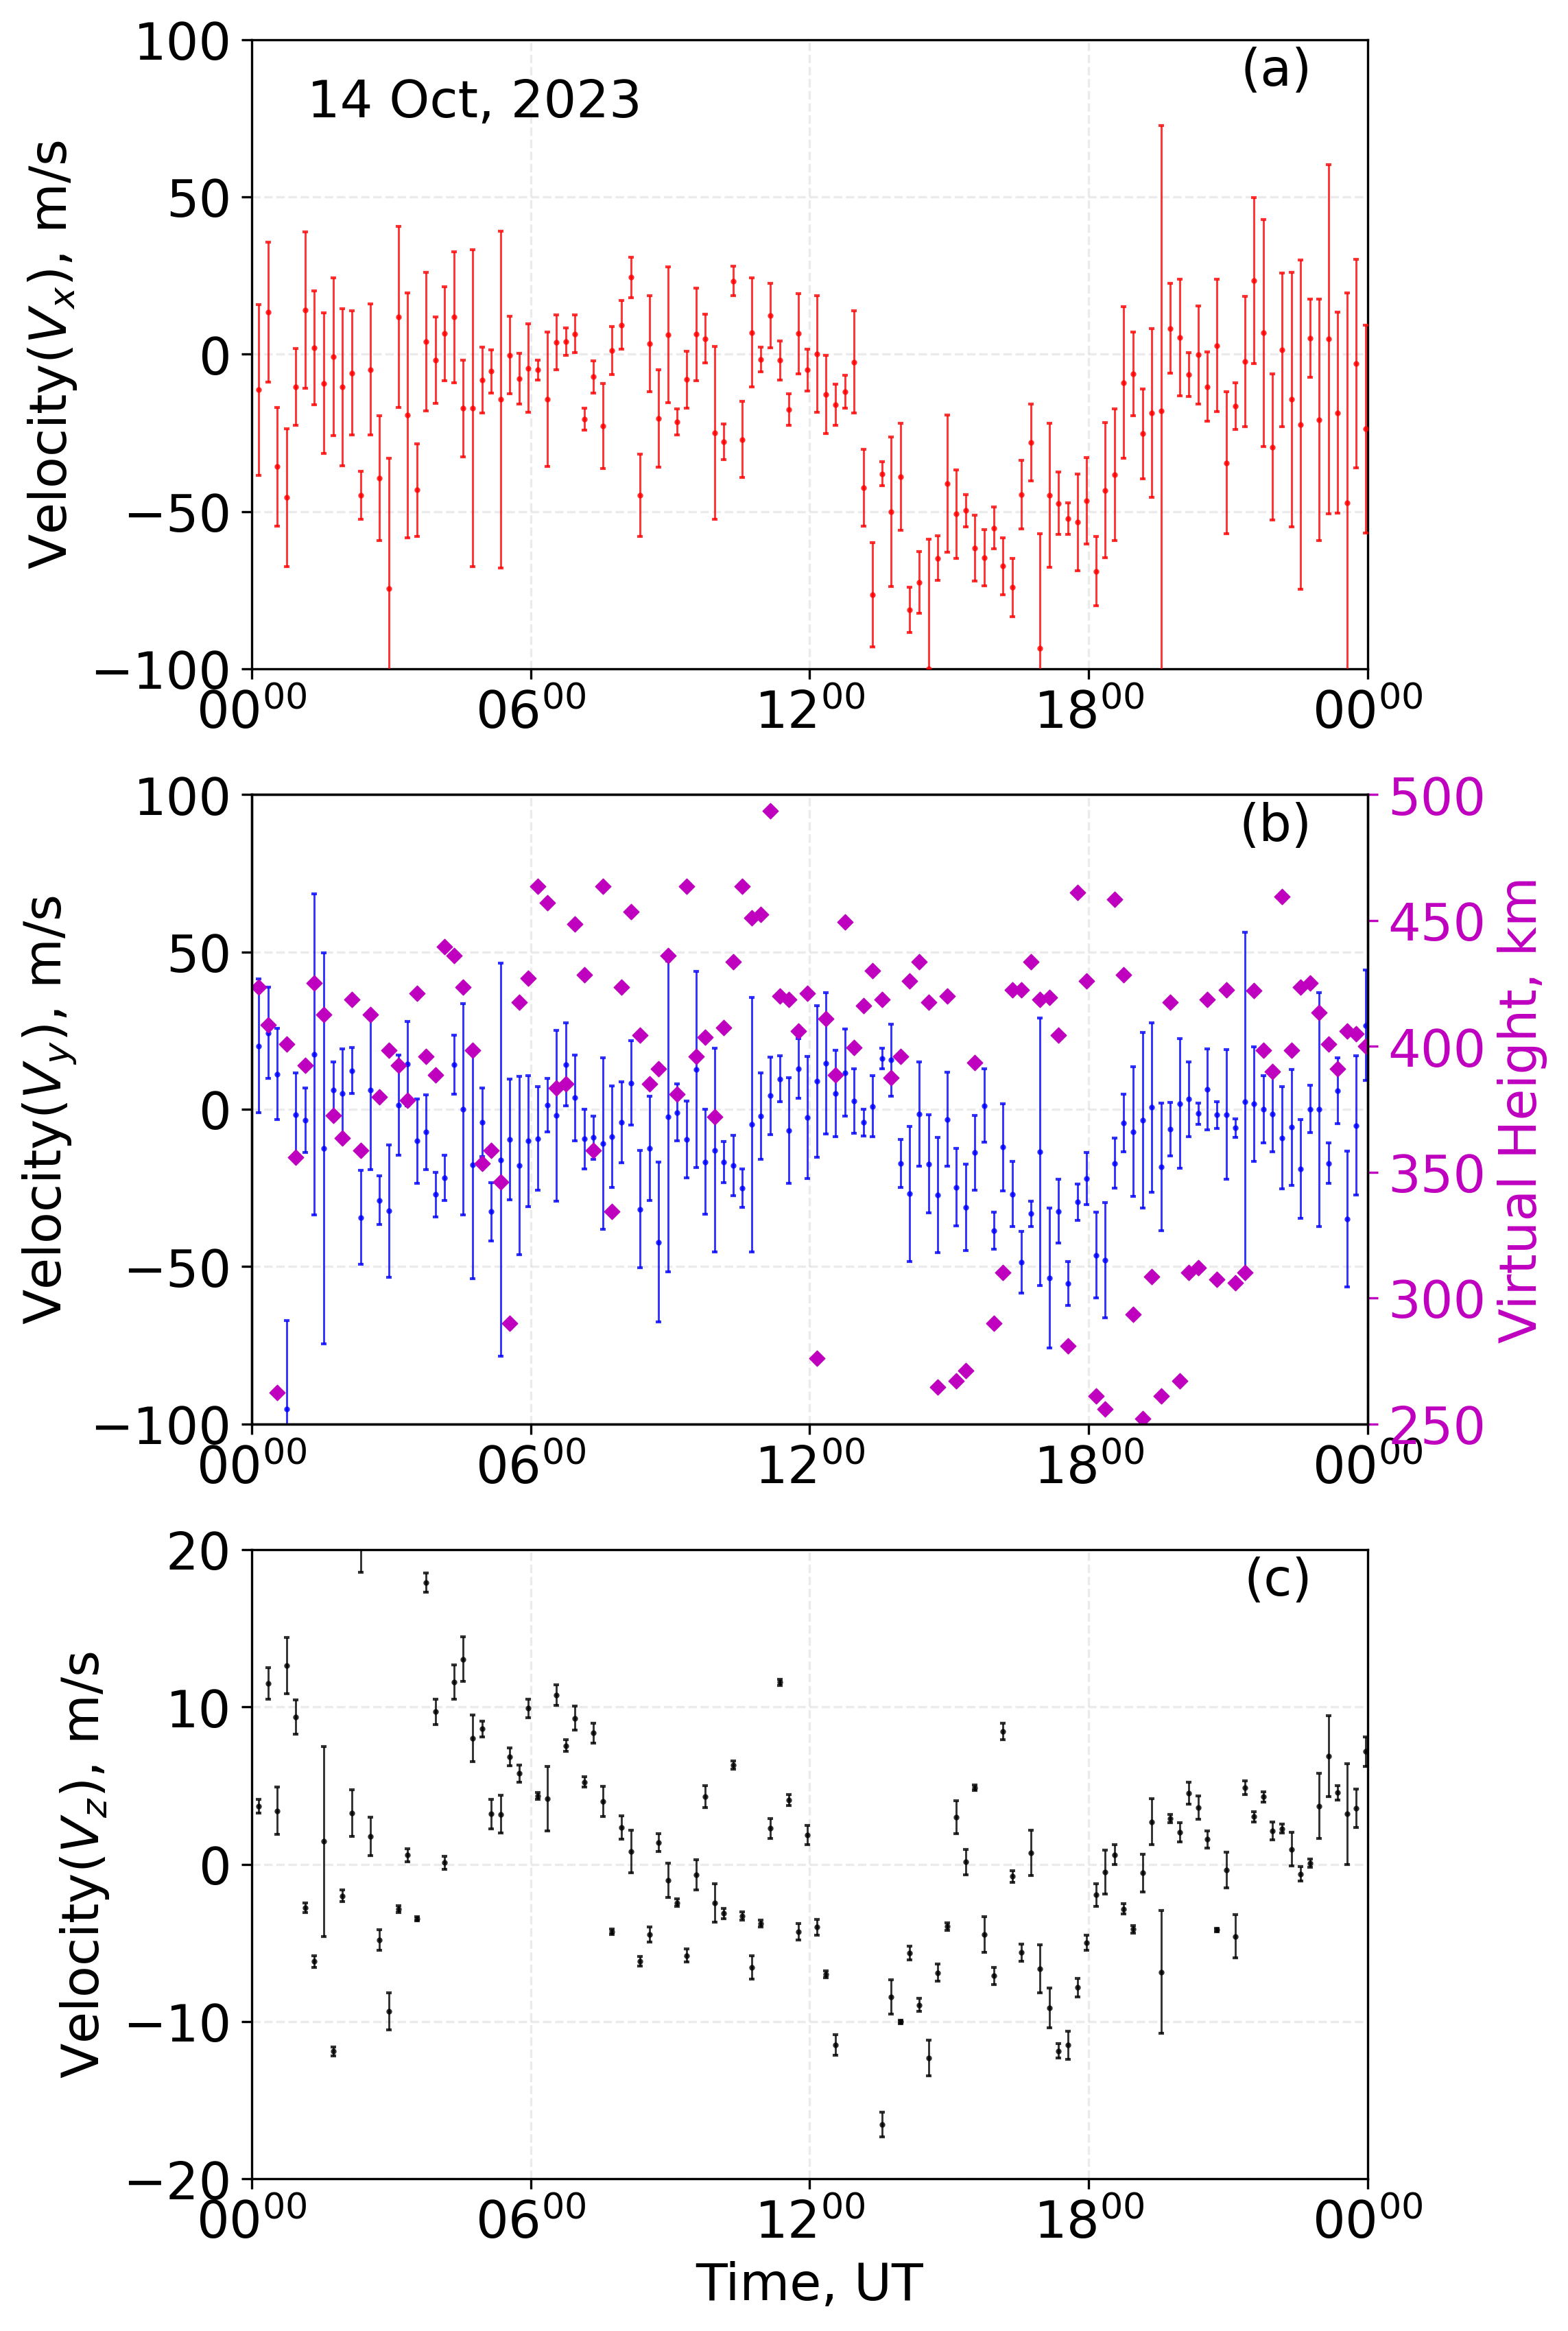
\includegraphics[width=0.72\linewidth,height=4.2cm,keepaspectratio]{stackplots_dvl.png}
  \end{center}
\end{frame}

% ----------------------------------------------------------------
\section{VIPIR Data}
% ----------------------------------------------------------------

\begin{frame}[fragile]{VIPIR RIQ File Structure}
  \begin{center}
  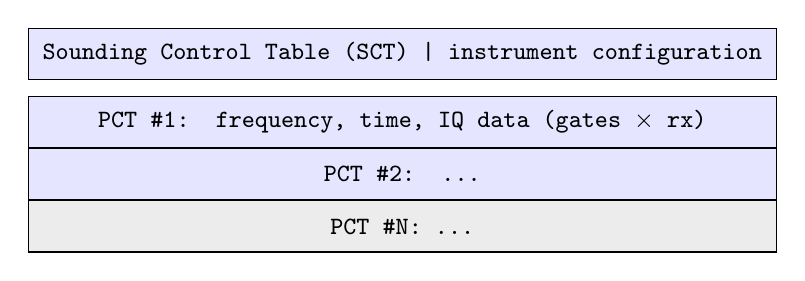
\begin{tikzpicture}[node distance=0mm,
    box/.style={draw,fill=blue!10,minimum width=9.5cm,minimum height=0.65cm,
                font=\ttfamily\small,align=center}]
    \node[box] (sct) {Sounding Control Table (SCT) — instrument configuration};
    \node[box,below=2mm of sct] (pct1) {PCT \#1: frequency, time, IQ data (gates $\times$ rx)};
    \node[box,below=0mm of pct1] (pct2) {PCT \#2: \ldots};
    \node[box,below=0mm of pct2,fill=gray!15] (pctN) {PCT \#N: \ldots};
  \end{tikzpicture}
  \end{center}
  \begin{lstlisting}
from pynasonde.vipir.riq.parsers.read_riq import RiqDataset, VIPIR_VERSION_MAP

riq = RiqDataset.create_from_file(
    "data/WI937_20220821.RIQ",
    vipir_config=VIPIR_VERSION_MAP.configs[1],   # older WI937 format
)
print(f"Gates  : {riq.sct.timing.gate_count}")   # 960
print(f"Freqs  : {riq.sct.frequency.base_steps}")
  \end{lstlisting}
\end{frame}

\begin{frame}[fragile]{VIPIR — Echo Extraction}
  \begin{columns}
  \column{0.50\textwidth}
    \begin{lstlisting}
from pynasonde.vipir.riq.echo \
    import EchoExtractor

extractor = EchoExtractor(
  sct=riq.sct,
  pulsets=riq.pulsets,
  snr_threshold_db=3.0,
  min_rx_for_direction=3,
).extract()

df = extractor.to_dataframe()
    \end{lstlisting}
  \column{0.46\textwidth}
    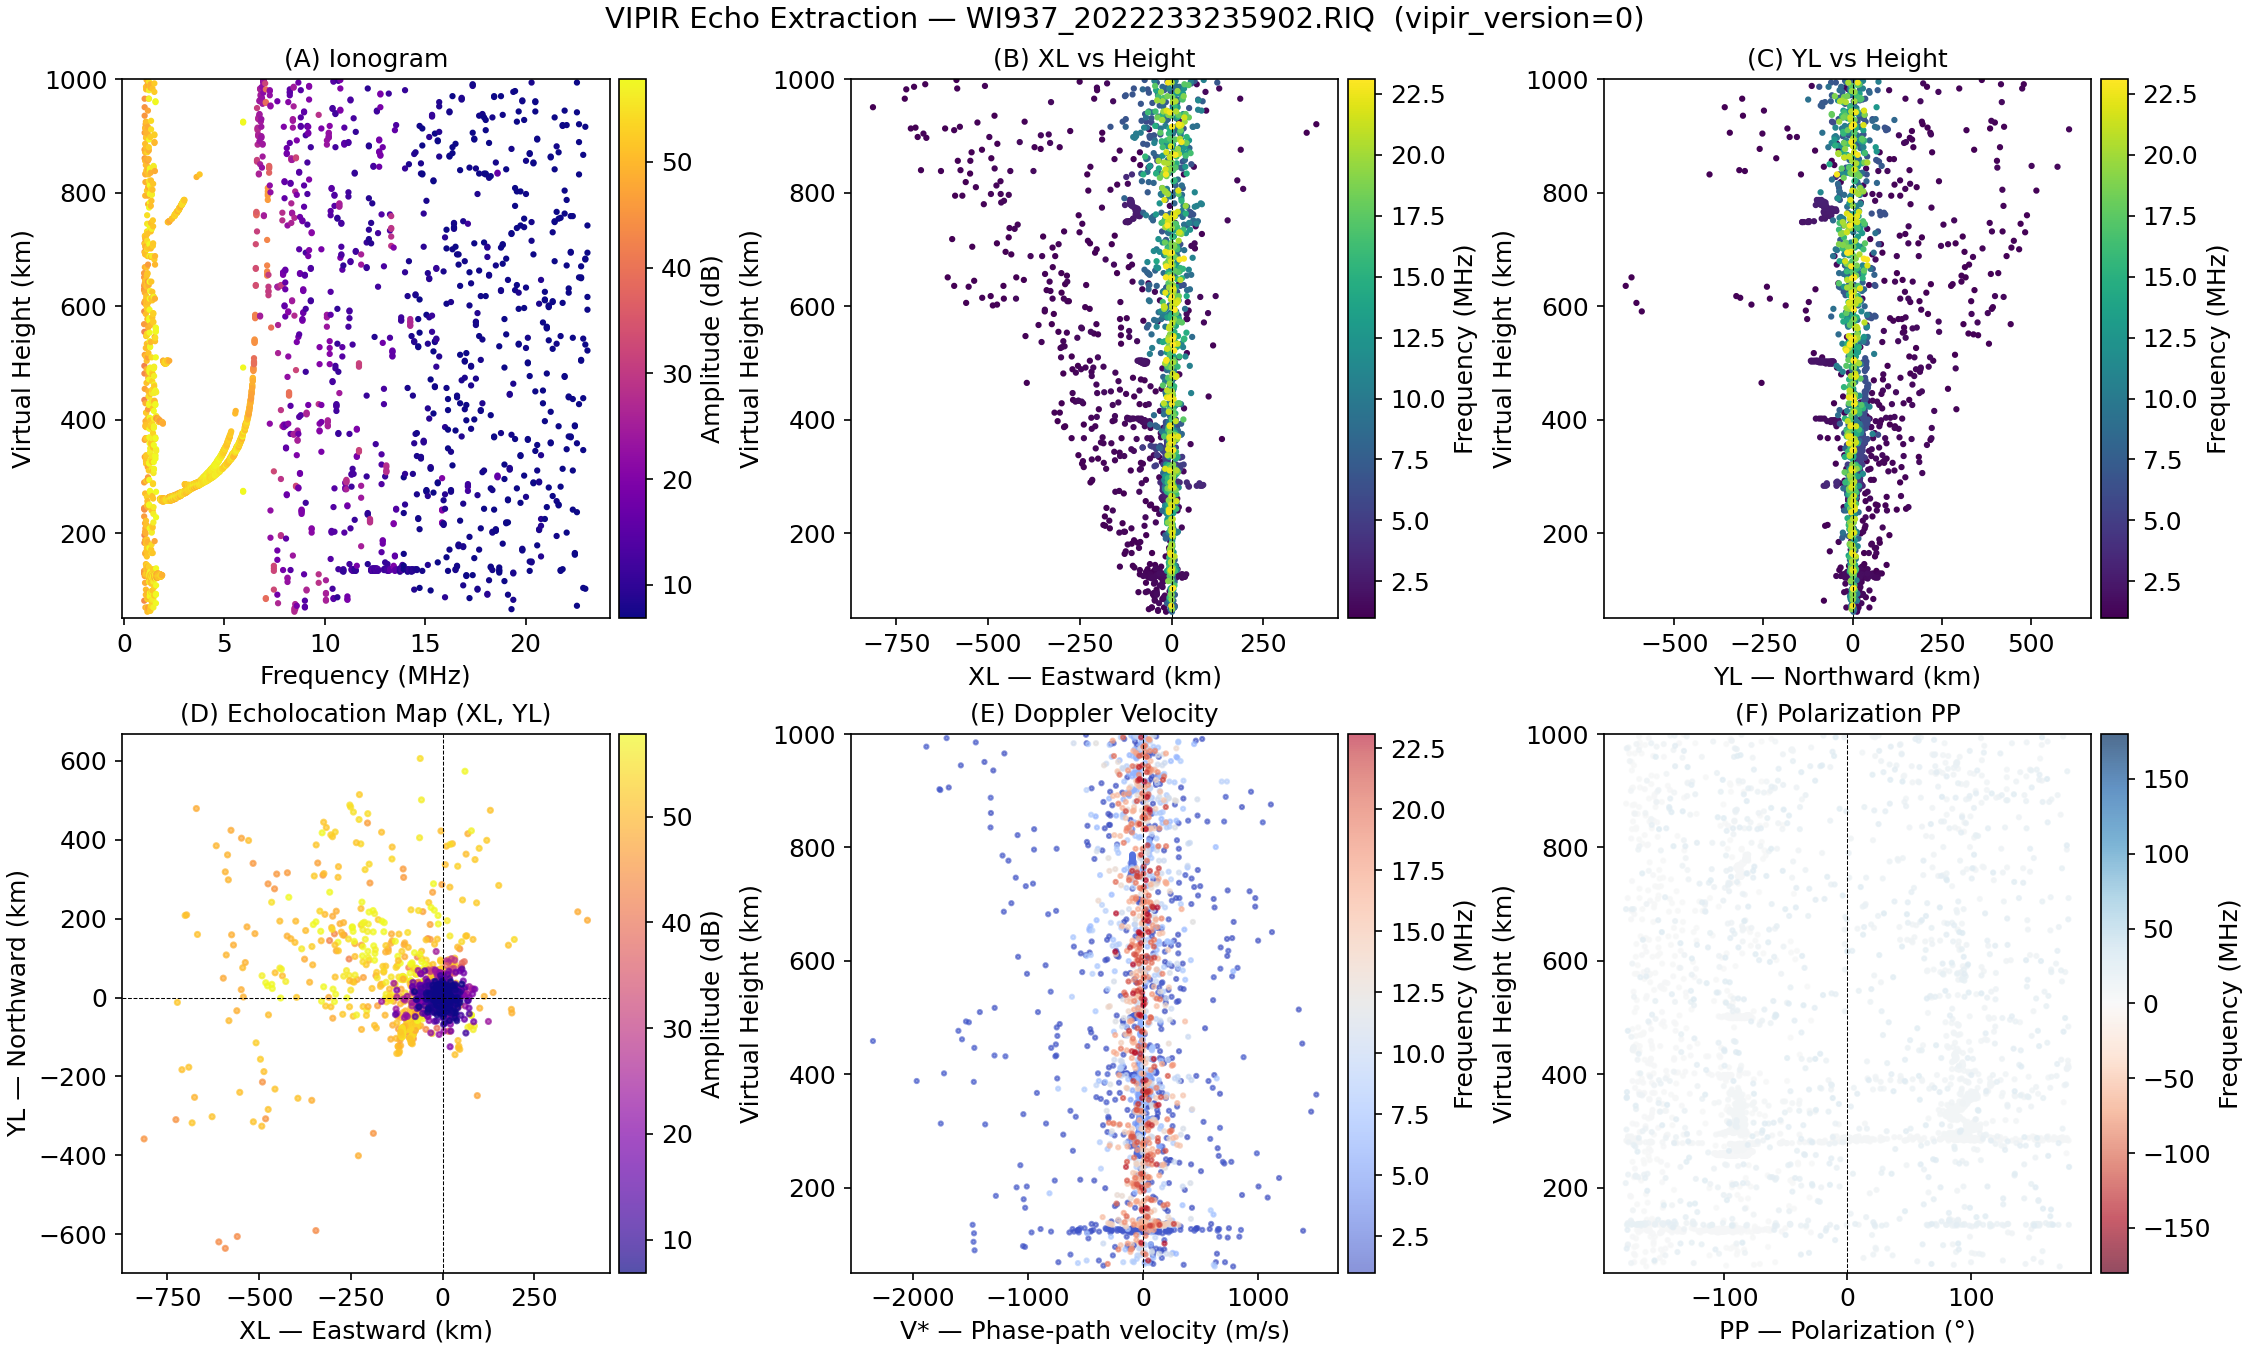
\includegraphics[width=\linewidth,height=4.2cm,keepaspectratio]{echo_extraction_wi937.png}
  \end{columns}
  {\small Six-panel diagnostic: ionogram, XL/YL direction cosines, Doppler V*, PP polarization.}
\end{frame}

\begin{frame}[fragile]{VIPIR — Ionogram Filter}
  \begin{columns}
  \column{0.50\textwidth}
    \begin{lstlisting}
from pynasonde.vipir.riq.parsers.\
    filter import IonogramFilter

filtered = IonogramFilter(
  snr_threshold_db=6.0,
  ep_threshold_deg=30.0,
  use_dbscan=True,
  use_ransac=True,
).fit(df)
    \end{lstlisting}
    \vspace{0.2cm}
    {\small 6 stages: RFI → EP → multi-hop → DBSCAN → RANSAC → temporal coherence}
  \column{0.46\textwidth}
    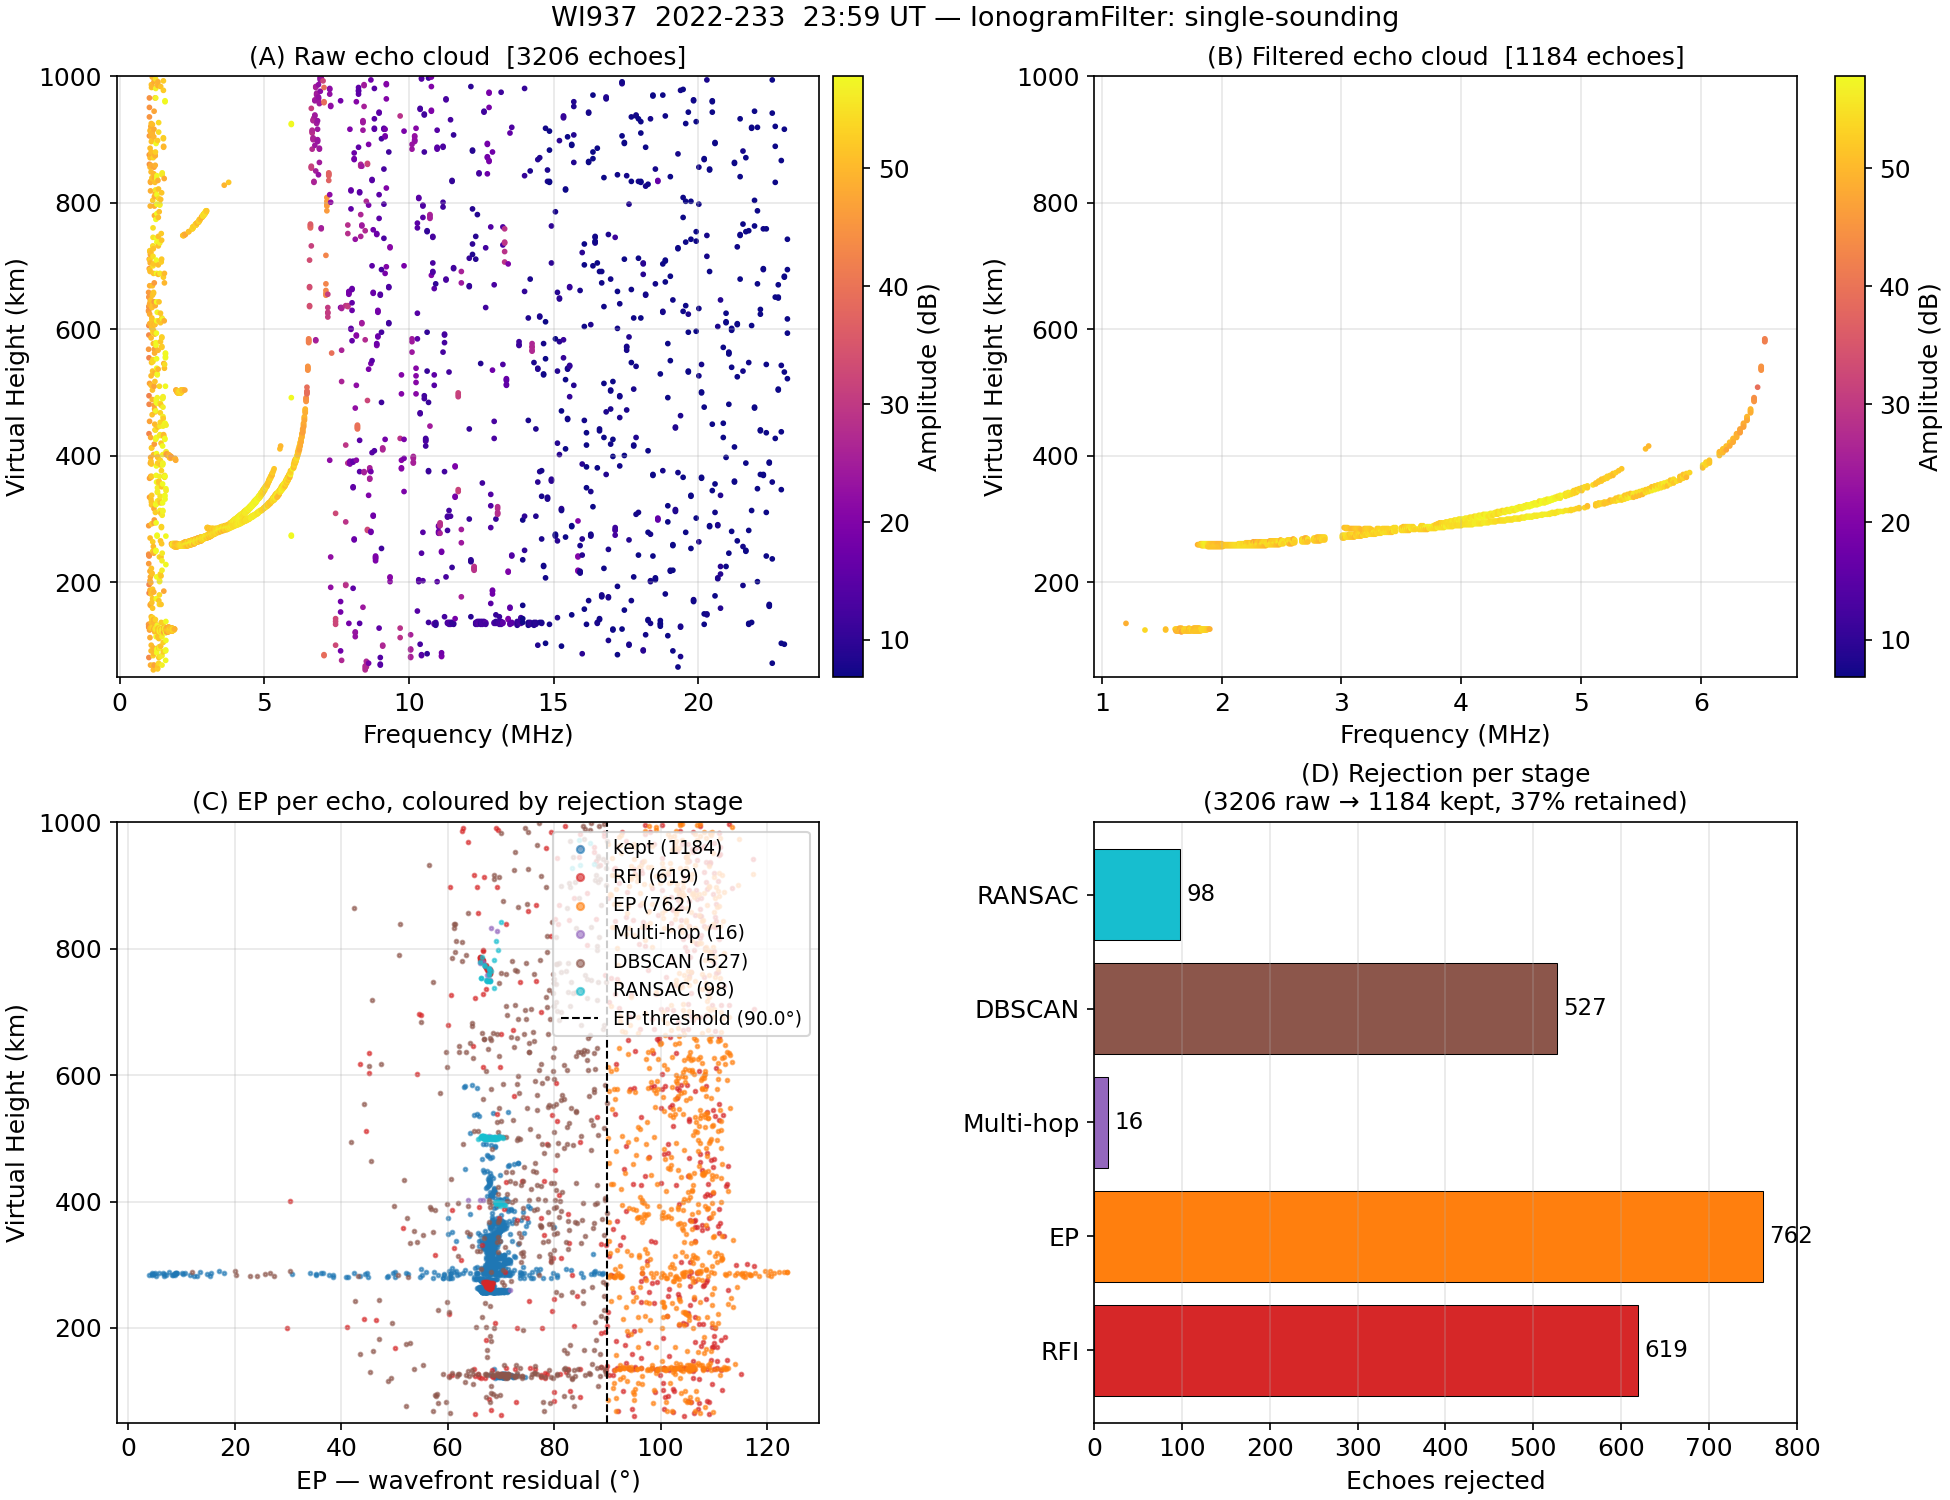
\includegraphics[width=\linewidth]{ionogram_filter_wi937.png}
  \end{columns}
\end{frame}

\begin{frame}{VIPIR — FTI (Frequency–Time Interval)}
  \begin{center}
    \includegraphics[width=0.82\linewidth,height=5.2cm,keepaspectratio]{fti.WI937.2022j.png}
  \end{center}
  {\small O-mode power FTI panels from a full day of WI937 NGI ionograms.}
\end{frame}

% ----------------------------------------------------------------
\section{Ionospheric Analysis}
% ----------------------------------------------------------------

\begin{frame}[fragile]{O/X Mode Separation}
  \begin{columns}
  \column{0.52\textwidth}
    \begin{lstlisting}
from pynasonde.vipir.analysis \
    import PolarizationClassifier

clf = PolarizationClassifier(
  o_mode_sign=-1,       # N. hemisphere
  pp_ambiguous_threshold_deg=20,
)
pol = clf.fit(filtered_df)
print(pol.summary())
# O=412  X=388  ambiguous=54

o_df = pol.o_mode_df()
    \end{lstlisting}
  \column{0.44\textwidth}
    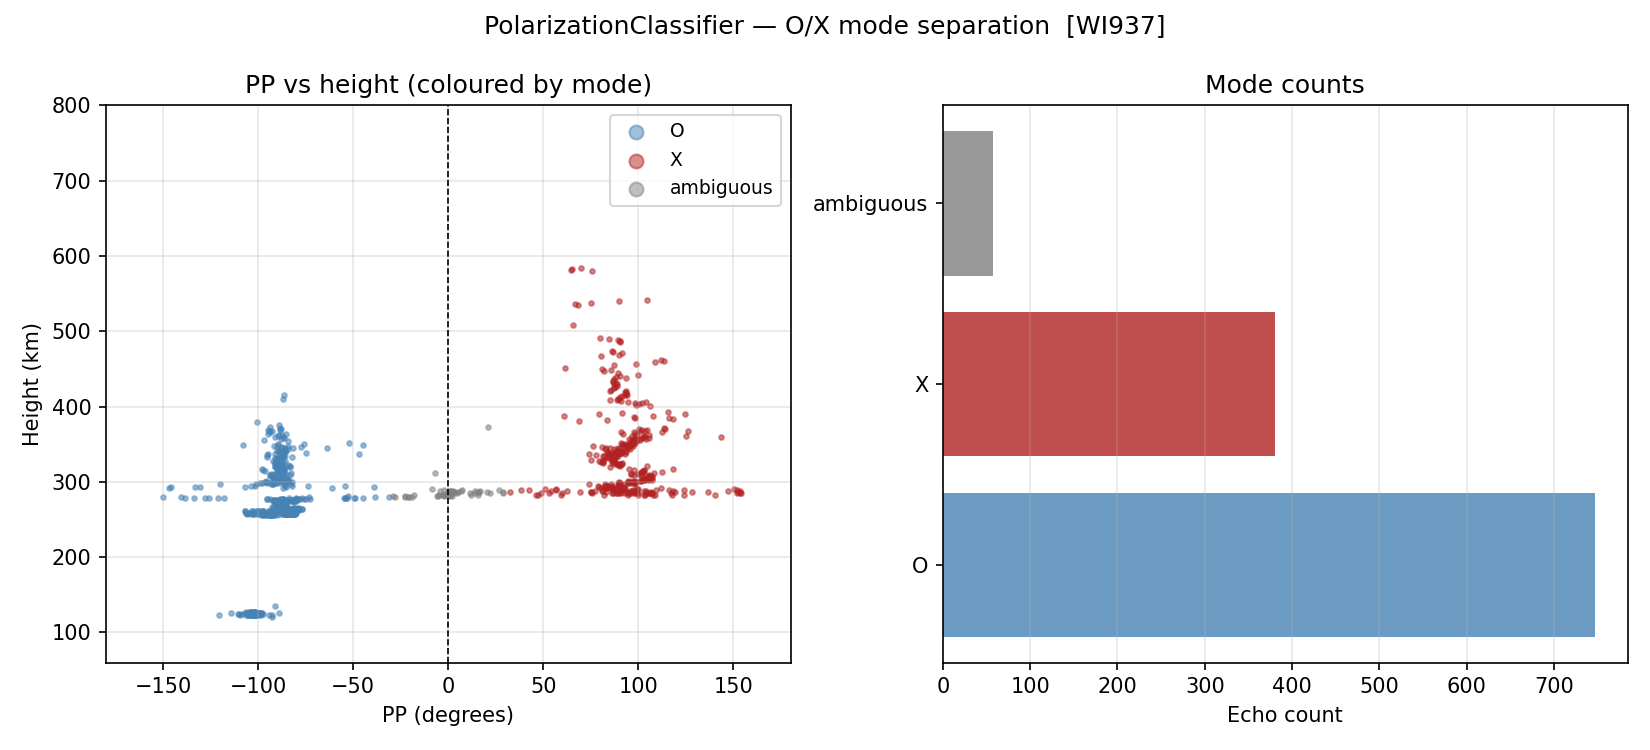
\includegraphics[width=\linewidth]{analysis_polarization.png}
  \end{columns}
\end{frame}

\begin{frame}[fragile]{True Height Inversion → N(h)}
  \begin{columns}
  \column{0.50\textwidth}
    \begin{lstlisting}
from pynasonde.vipir.analysis \
    import TrueHeightInversion

inv = TrueHeightInversion()
edp = inv.fit_from_df(o_df)

print(edp.summary())
# foF2=8.12 MHz
# hmF2=287.4 km
# NmF2=8.2e5 cm^-3

edp.plot()
    \end{lstlisting}
  \column{0.46\textwidth}
    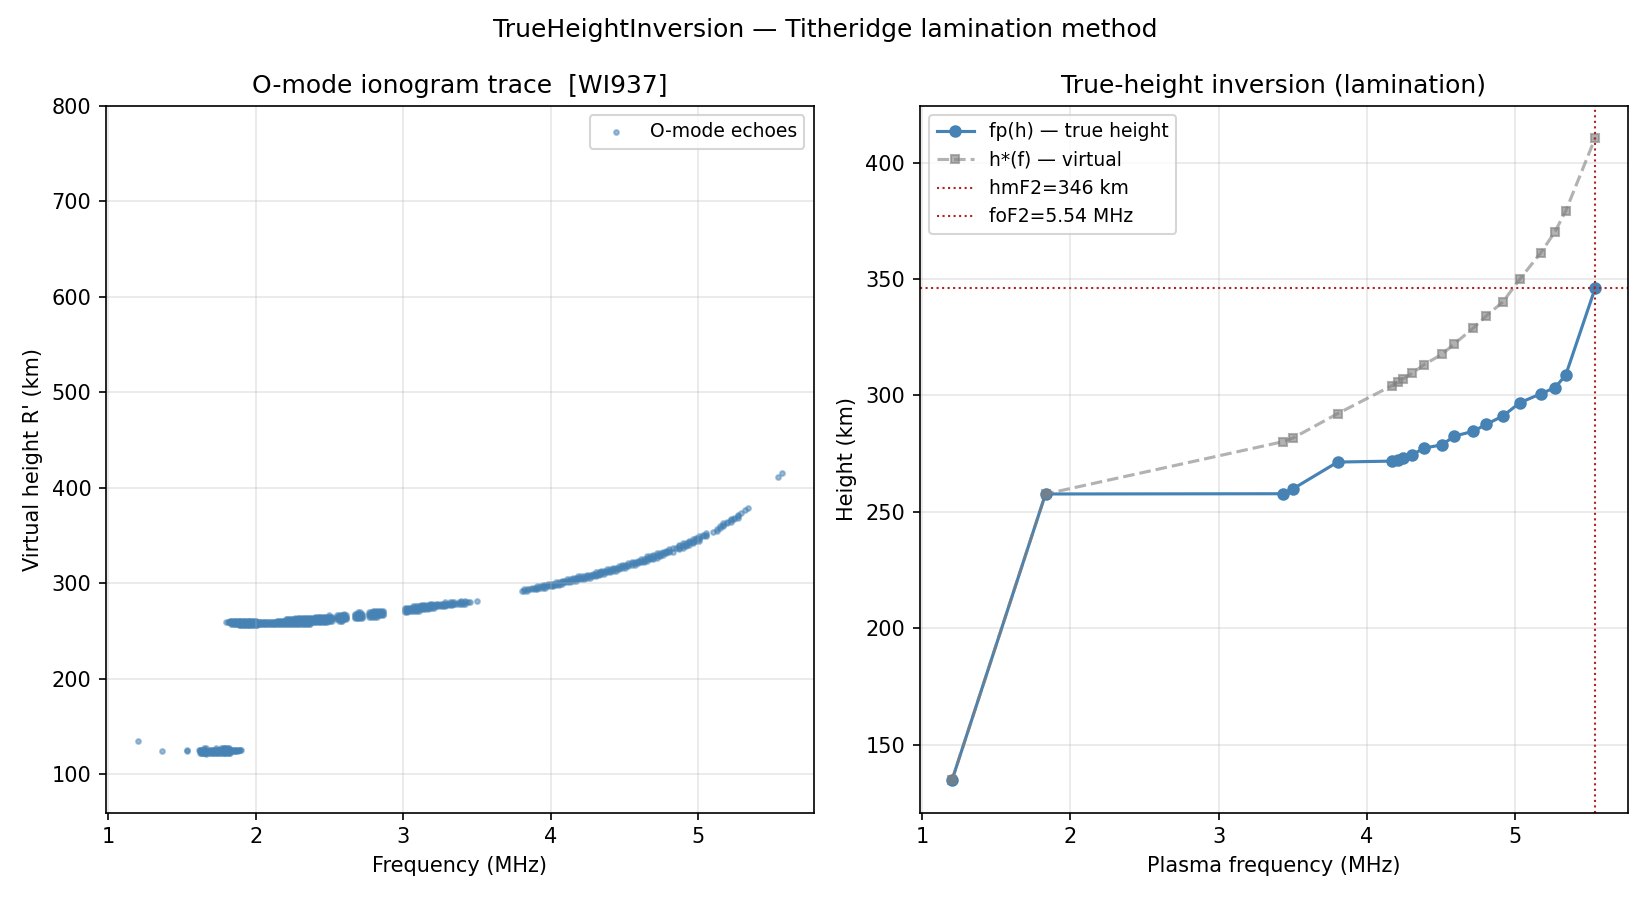
\includegraphics[width=\linewidth]{analysis_inversion.png}
  \end{columns}
\end{frame}

\begin{frame}[fragile]{HF Absorption}
  \begin{columns}
  \column{0.52\textwidth}
    {\lstset{basicstyle=\ttfamily\scriptsize}
    \begin{lstlisting}
from pynasonde.vipir.analysis \
    import AbsorptionAnalyzer
import numpy as np

aa = AbsorptionAnalyzer()
# 1. LOF index (no calibration)
lof = aa.lof_absorption(df)
# 2. Differential O/X
diff = aa.differential_absorption(
    pol.annotated_df)
# 3. Height-resolved profile
prof = aa.absorption_profile(
  edp,
  nu_hz=lambda h: 1e6*np.exp(-h/8))
    \end{lstlisting}}
  \column{0.44\textwidth}
    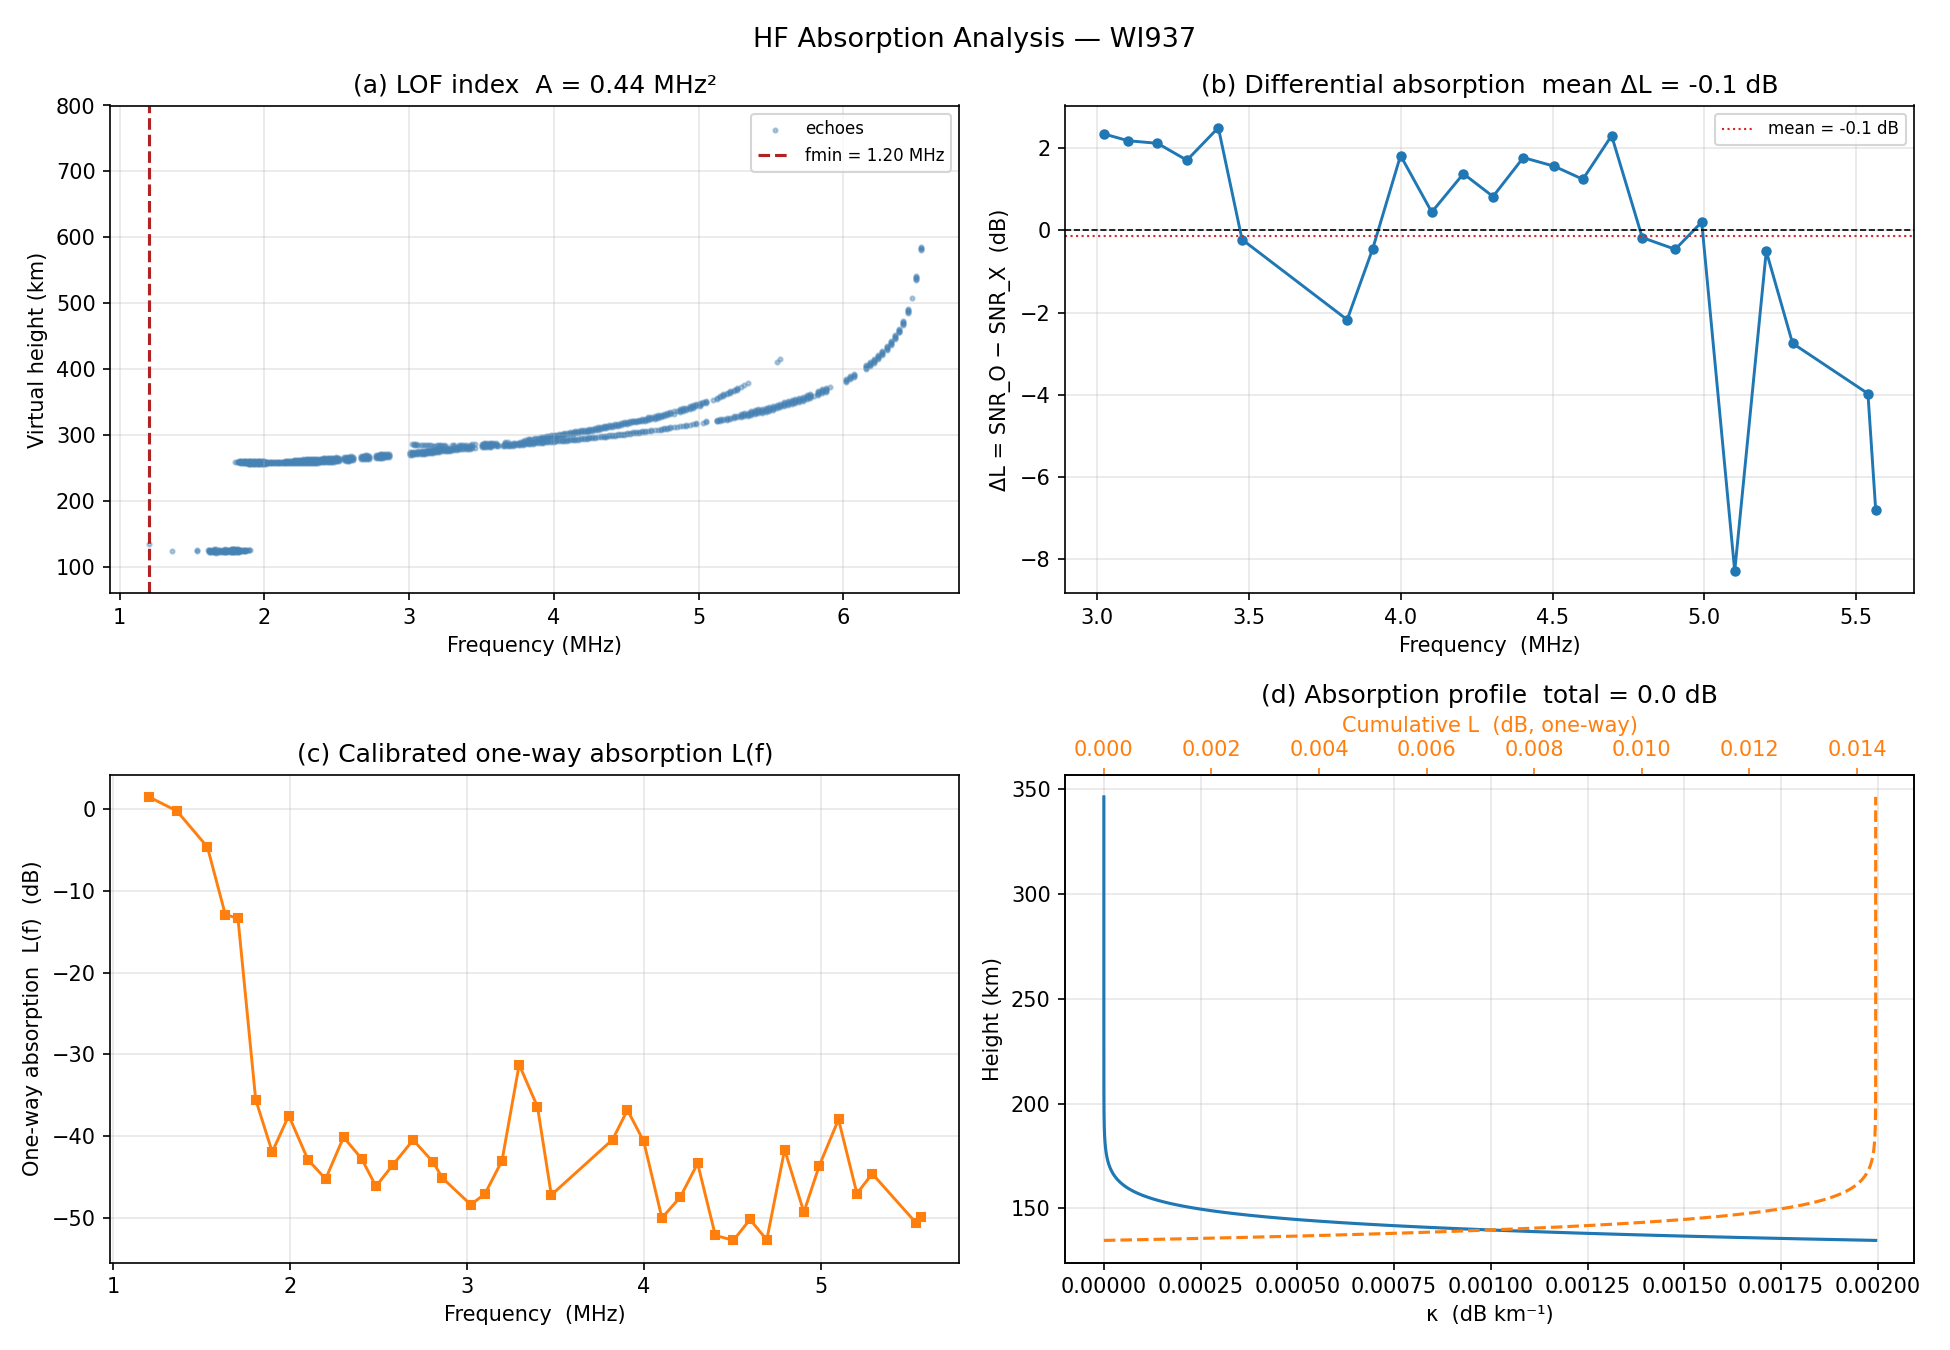
\includegraphics[width=\linewidth,height=4.0cm,keepaspectratio]{analysis_absorption.png}
  \end{columns}
\end{frame}

% ----------------------------------------------------------------
\section{Es Layer Imaging}
% ----------------------------------------------------------------

\begin{frame}{Sporadic-E — Why Higher Resolution?}
  \begin{columns}
  \column{0.55\textwidth}
    \begin{itemize}
      \item Es: thin metallic-ion layer at 90--130~km ($<$1~km thick)
      \item VIPIR native gate $r_0 = 1.499$~km — \textbf{cannot resolve thin layers}
      \item \textbf{Capon cross-spectrum imaging} (Liu et al.\ 2023):
            \textbf{10× finer resolution}, no extra hardware
      \item Key: FFT of range profile as spatial frequency array;
            minimum-variance beamforming in \emph{range space}
    \end{itemize}
  \column{0.42\textwidth}
    \begin{block}{Effective resolution}
      \[
        \Delta r = \frac{r_0}{K}
      \]
      \begin{tabular}{lcc}
        \toprule
        Instrument & $r_0$ & $\Delta r$ (K=10) \\
        \midrule
        WISS  & 3.84 km & 384 m \\
        VIPIR & 1.499 km & 150 m \\
        \bottomrule
      \end{tabular}
    \end{block}
  \end{columns}
\end{frame}

\begin{frame}{Es Imaging Sanity Check — Liu et al.\ Fig.~1}
  \begin{center}
    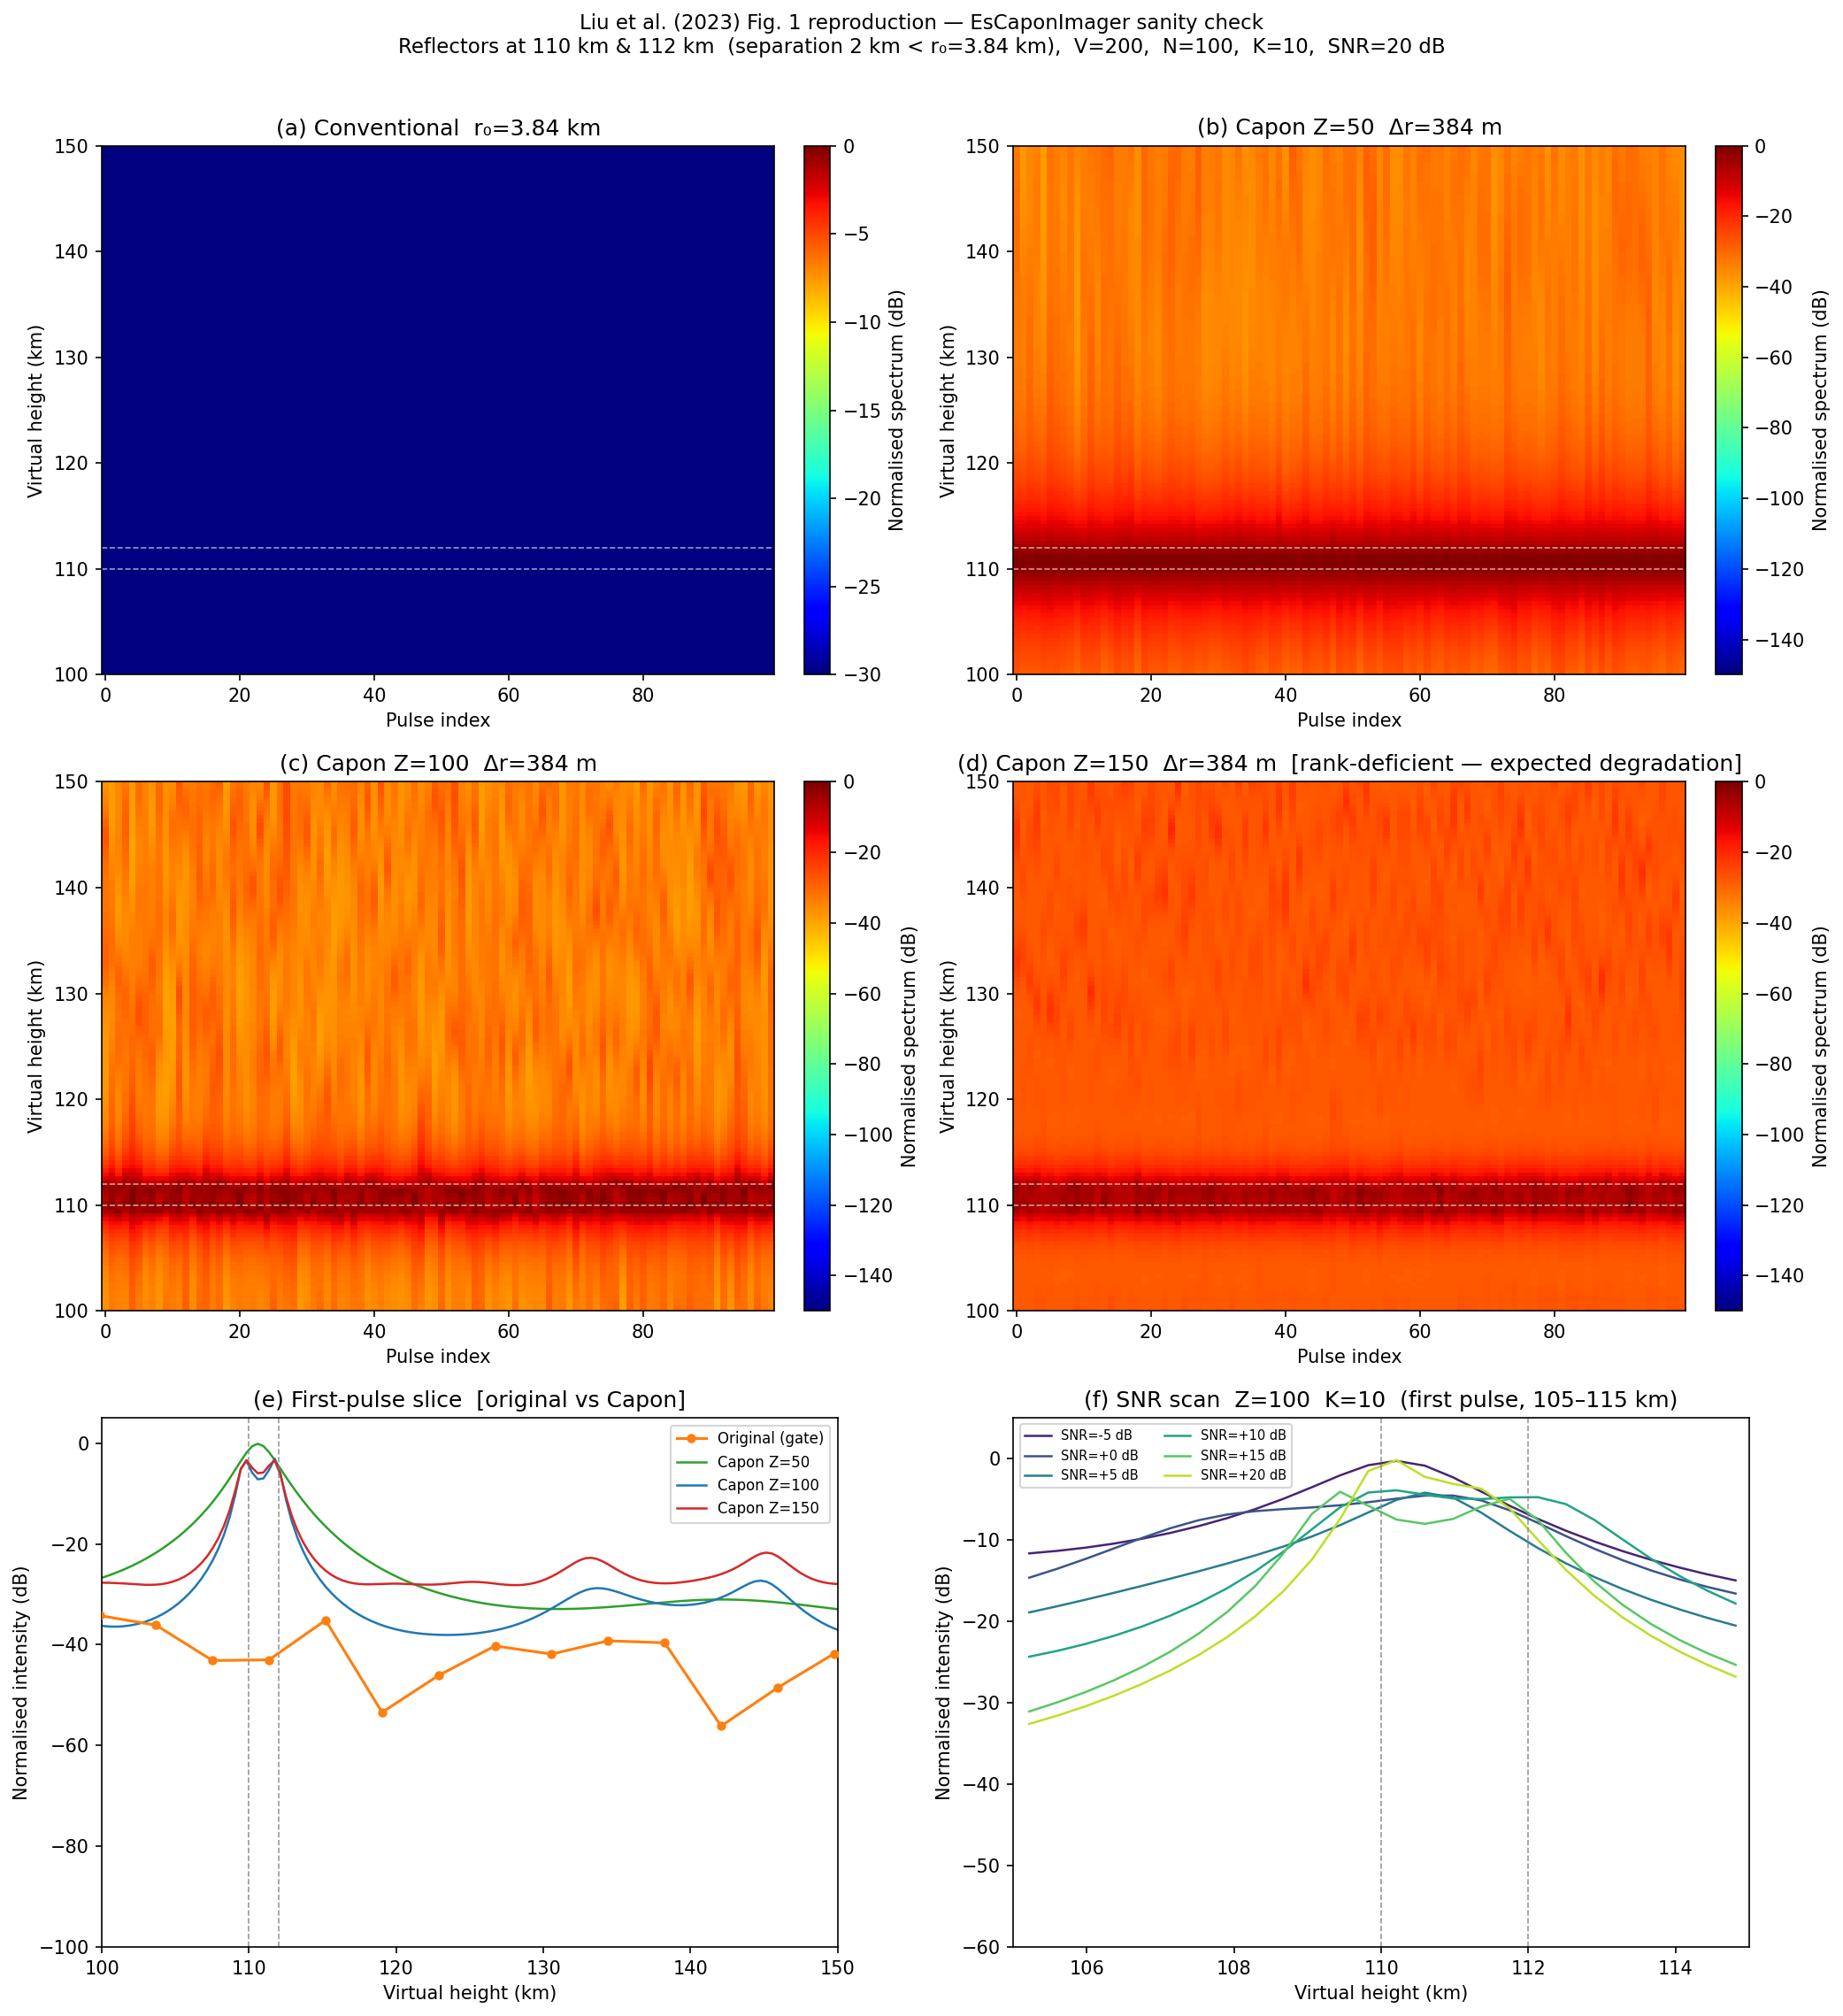
\includegraphics[width=0.85\linewidth,height=5.2cm,keepaspectratio]{es_imaging_sanity_check.png}
  \end{center}
  {\small Synthetic two-layer test (110 + 112~km).
   $Z=50$: unresolved. $Z=100$: peaks at 109.8 \& 111.7~km ($<$0.3~km error).
   $Z=150$: rank-deficient (matches paper Fig.~1d).}
\end{frame}

\begin{frame}[fragile]{Es Imaging — Single File}
  \begin{lstlisting}
from pynasonde.vipir.analysis import EsCaponImager

imager = EsCaponImager(
    n_subbands=100,         # Z  (Z <= (V+1)/2 recommended)
    resolution_factor=10,   # K  (no singularity constraint)
    gate_spacing_km=1.499,  # VIPIR native gate r0
    gate_start_km=90.0,
)
result = imager.fit(iq_cube)   # (pulses, gates) or (pulses, gates, rx)
print(result.summary())
# EsImagingResult: Z=100  K=10  r0=1.499 km -> Dr=0.150 km
result.plot(snapshot=0)
  \end{lstlisting}
\end{frame}

\begin{frame}{Es Imaging — Single File Result}
  \begin{center}
    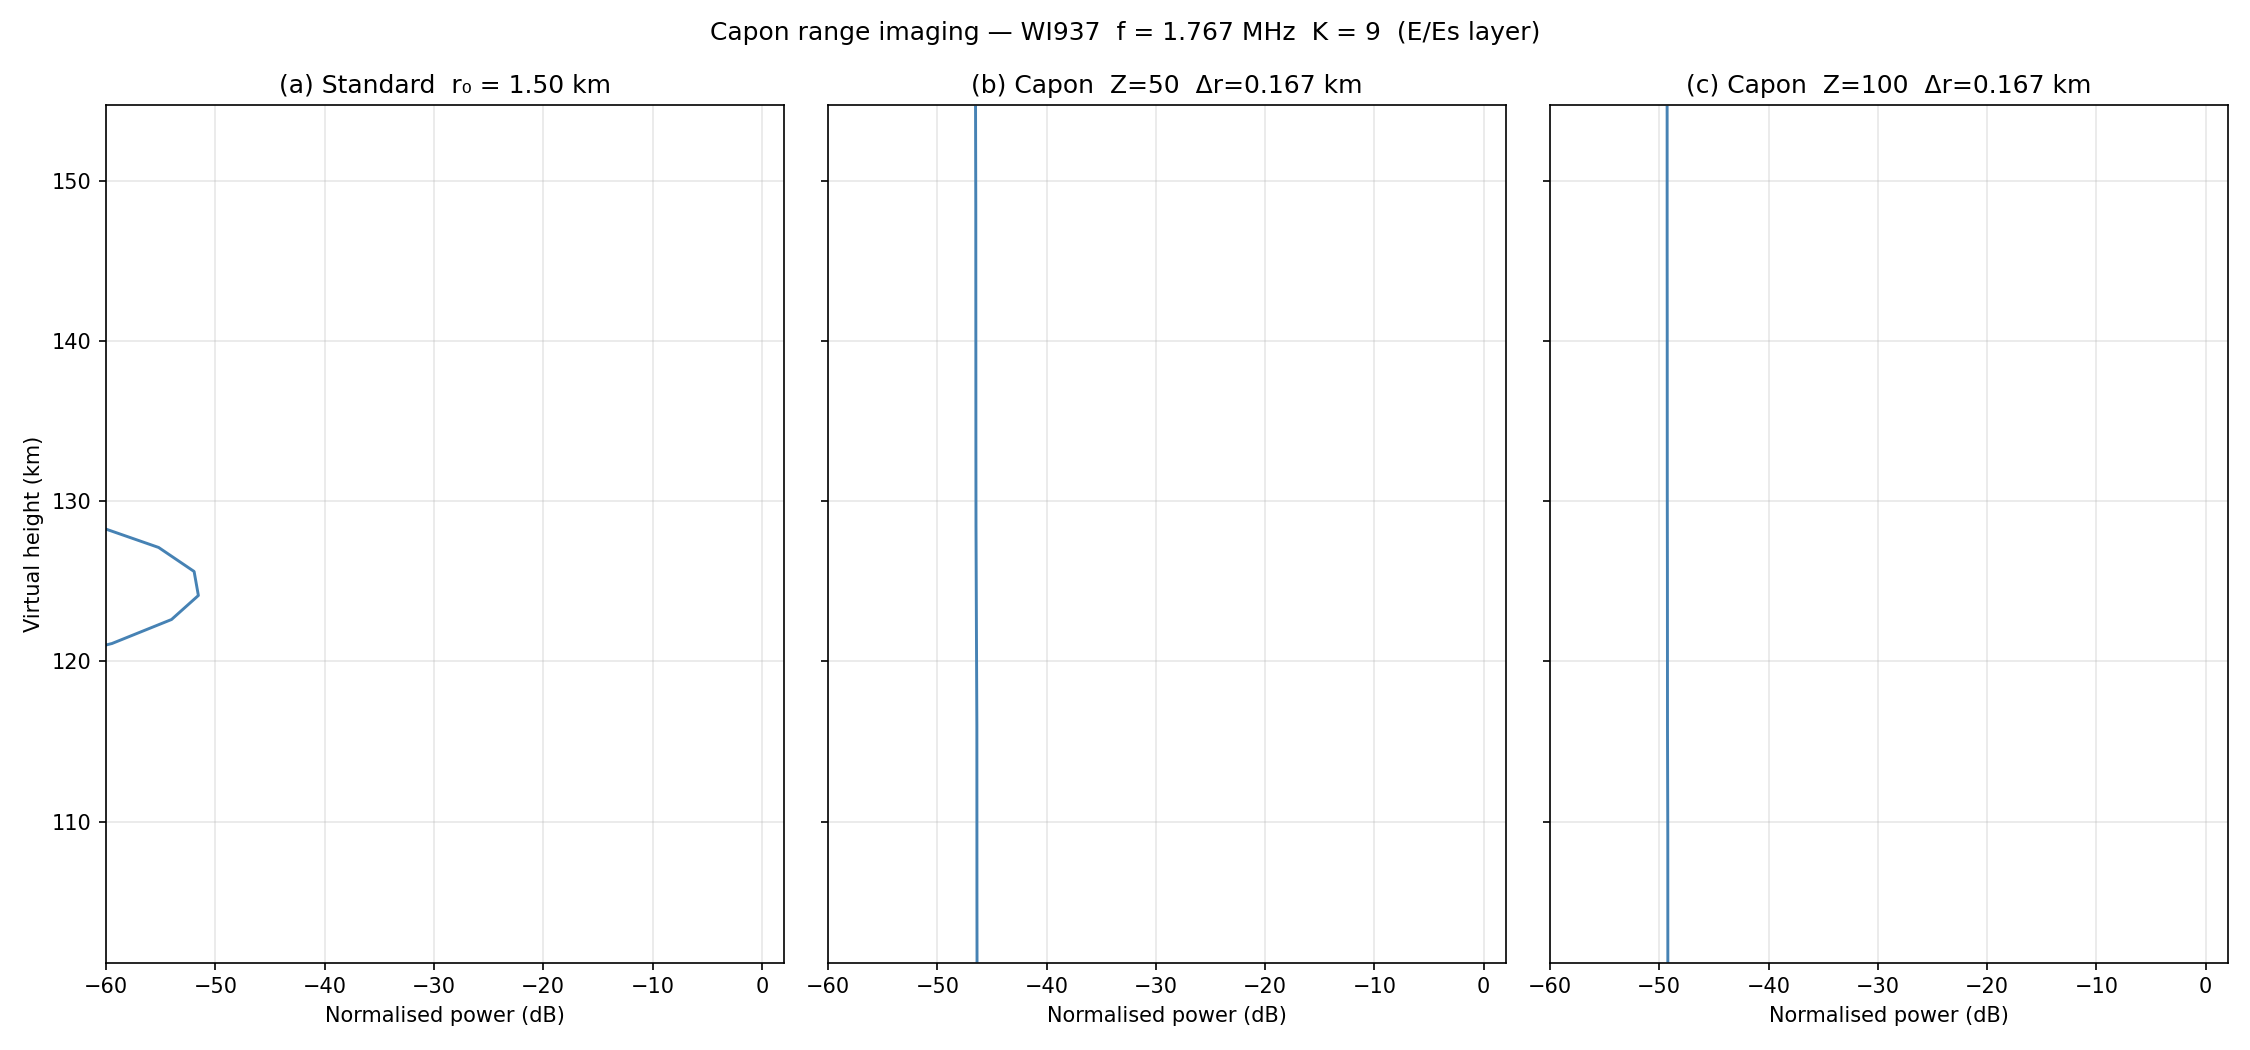
\includegraphics[width=0.72\linewidth]{analysis_es_imaging.png}
  \end{center}
\end{frame}

\begin{frame}[fragile]{Es Imaging — Multi-File A+B+C}
  When only 4 pulses/file: combine 8 files × 4 pulses × 8 Rx = 256 samples:
  \begin{lstlisting}
from pynasonde.vipir.analysis import RiqAggregator
import glob

files = sorted(glob.glob("data/20230601_05??.RIQ"))[:8]

agg = RiqAggregator(
    n_subbands=100, resolution_factor=10,
    output_mode="slow_rti",   # one column per file
)
result = agg.fit(files, freq_target_khz=5000.0)
result.plot()
  \end{lstlisting}
  \begin{block}{SNR improvement}
    \small Option A (8 Rx coherent): $+9$~dB \;|\;
           Option B (4-pulse avg): $\div 4$ var \;|\;
           Option C (8-file stack): $\div 8$ var \;$\Rightarrow$\; $\sim$24~dB total
  \end{block}
\end{frame}

\begin{frame}{Es Imaging — Slow RTI (A+B+C)}
  \begin{center}
    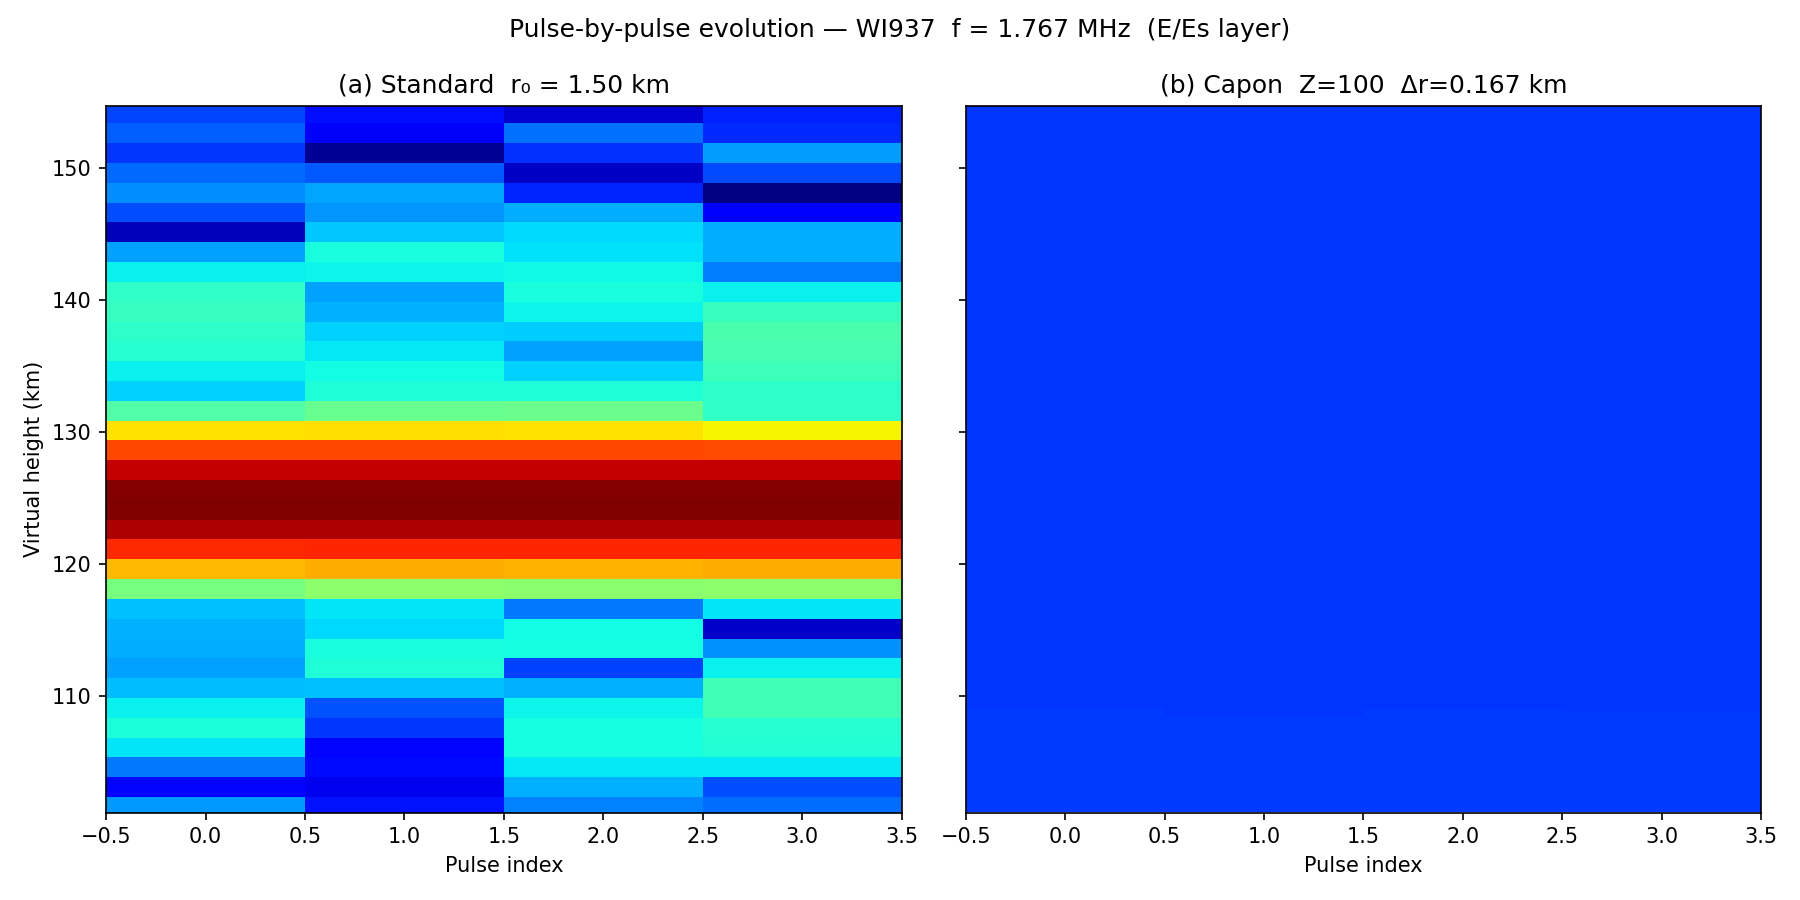
\includegraphics[width=0.80\linewidth]{analysis_es_imaging_rti.png}
  \end{center}
  {\small Slow RTI: one column per file ($\sim$1~min cadence).
  Each column is a Capon pseudospectrum averaged over Option A+B.}
\end{frame}

% ----------------------------------------------------------------
\section{Hands-On Exercises}
% ----------------------------------------------------------------

\begin{frame}{Hands-On Exercises}
  \begin{columns}
  \column{0.50\textwidth}
    \textbf{DIGISONDE}
    \begin{enumerate}\small
      \item Load a \texttt{.SAO} file. Print foF2 and hmF2.
      \item Build a daily isodensity contour from multiple SAO files.
      \item Load a \texttt{.DVL} file and plot the Vz time series.
      \item Load a \texttt{.DFT} file and produce a Doppler waterfall.
    \end{enumerate}
  \column{0.48\textwidth}
    \textbf{VIPIR}
    \begin{enumerate}\small
      \setcounter{enumi}{4}
      \item Load a WI937 RIQ file; print gate count and frequency range.
      \item Run \texttt{IonogramFilter}. How many echoes survive?
      \item Separate O/X modes. What fraction is O-mode?
      \item Run \texttt{TrueHeightInversion}. What is foF2?
      \item Run \texttt{EsCaponImager} with $Z=100$, $K=10$. Is there a thin Es layer?
      \item Compute the LOF absorption index.
    \end{enumerate}
  \end{columns}
\end{frame}

% ----------------------------------------------------------------
\section{Summary}
% ----------------------------------------------------------------

\begin{frame}{Summary — I/O Layer (1/2)}
  \begin{columns}
  \column{0.48\textwidth}
    \textbf{DIGISONDE I/O — 8 file formats}
    \begin{itemize}\small
      \item \texttt{SaoExtractor} — SAO 4.3/5.0: N(h) + scaled params
      \item \texttt{RsfExtractor} — direction-coded ionogram + directogram
      \item \texttt{SbfExtractor} — SBF binary raw soundings
      \item \texttt{DftExtractor} — Doppler waterfall + spectra
      \item \texttt{DvlExtractor} — drift velocities Vx, Vy, Vz
      \item \texttt{SkyExtractor} — polar sky maps (az/zen)
      \item \texttt{EdpExtractor} — electron density profiles
      \item \texttt{SaoSummaryPlots}, \texttt{SkySummaryPlots}
    \end{itemize}
  \column{0.48\textwidth}
    \textbf{VIPIR I/O — 3 file formats}
    \begin{itemize}\small
      \item \texttt{RiqDataset} — SCT + PCT loader, \texttt{VIPIR\_VERSION\_MAP}
      \item \texttt{EchoExtractor} — 7-param echoes (h, A, V*, EP, PP, XL, YL)
      \item \texttt{IonogramFilter} — 6-stage: RFI, EP, multi-hop, DBSCAN, RANSAC, temporal
      \item \texttt{DataSource} — NGI/SDR NetCDF loader + data cube
      \item \texttt{AutoScaler} — noise profile, segment, binary trace
      \item \texttt{FullPipeline} — end-to-end RIQ $\to$ N(h) automation
    \end{itemize}
  \end{columns}
\end{frame}

\begin{frame}{Summary — Analysis Layer (2/2)}
  \begin{columns}
  \column{0.50\textwidth}
    \textbf{Analysis layer — 9 classes (all post-v1.0)}
    \begin{itemize}\small
      \item \texttt{PolarizationClassifier} — O/X via PP chirality
      \item \texttt{TrueHeightInversion} — Titheridge/POLAN $\to$ N(h)
      \item \texttt{AbsorptionAnalyzer} — LOF / O-X diff / $\kappa(z)$ profile
      \item \texttt{SpreadFAnalyzer} — range / freq / mixed classification
      \item \texttt{IrregularityAnalyzer} — $\alpha(h)$, outer scale, anisotropy
    \end{itemize}
  \column{0.46\textwidth}
    \vspace{0.15cm}
    \begin{itemize}\small
      \item \texttt{IonogramScaler} — foF2, foE, $h'$F, MUF
      \item \texttt{EsCaponImager} — Capon imaging ($\Delta r = 150$~m)
      \item \texttt{RiqAggregator} — A+B+C multi-file ($\sim$24~dB SNR)
      \item \texttt{NeXtYZInverter} — 3-D WSI + Hamiltonian ray-tracing
    \end{itemize}
    \vspace{0.3cm}
    \begin{block}{}
      \small
      \href{https://pynasonde.readthedocs.io}{pynasonde.readthedocs.io}\\
      \texttt{pip install pynasonde}
    \end{block}
  \end{columns}
\end{frame}

% ----------------------------------------------------------------
\begin{frame}[allowframebreaks]{References}
  \footnotesize
  \begin{itemize}
    \item Liu, T., Yang, G., \& Jiang, C. (2023). High-resolution sporadic E layer
          observation. \textit{Space Weather}, 21, e2022SW003195.
    \item Titheridge, J.\ E. (1967). A new method for the analysis of ionospheric
          $h'(f)$ records. \textit{JATP}, 29, 763--778.
    \item Zabotin, N.\ A., Wright, J.\ W., \& Zhbankov, G.\ A. (2006). NeXtYZ.
          \textit{Radio Science}, 41, RS6S32.
    \item Grubb, R.\ N., et al.\ (2011). New science with the new VIPIR ionosonde.
          \textit{Radio Science}.
    \item Reinisch, B.\ W., et al.\ (1997). The Digisonde 4D. \textit{JASTP}, 59, 2181--2204.
    \item Davies, K. (1990). \textit{Ionospheric Radio}. Peter Peregrinus.
  \end{itemize}
\end{frame}

\end{document}
